\documentclass[14pt]{extreport}

% \usepackage[utf8]{inputenc} % ignore with LuaLaTeX

% **********************************************************
%                        PACKAGES
% **********************************************************

\usepackage[letterpaper, hmargin=1.5cm, top=3cm, bottom=2cm, headheight=17pt, headsep=1cm]{geometry}
\usepackage{blindtext}  % for creating random paragraphs
\usepackage{fancyhdr}   % for header and footer
\usepackage{titlesec}   % formats section titles 
%\usepackage[Lenny]{fncychap}
\usepackage[T1]{fontenc}
\usepackage{fontspec}
\usepackage[bitstream-charter]{mathdesign} % alternative nice font 
\usepackage{amsmath}    % math package
%\usepackage{amssymb}   
\usepackage{amsthm}     % math theorems
\usepackage{empheq}     % emphasizing/boxing equations
\usepackage{textcomp}   % load this before gensym to avoid warnings
\usepackage{gensymb}    % general symbols
\usepackage{enumitem}   % formatting enumerate and itemize environments
\usepackage{graphicx}   % for figures/images
\usepackage{longtable}  % for allowing tables to span onto another page
\usepackage{wrapfig}    % 
\usepackage{float}      % making figures floats with [H]
\usepackage{multicol, multirow} % to make multiple columns/rows
\usepackage{caption}    % formatting figure/table captions
\usepackage{hyperref}   % formmatting hyperlinks and other links
\usepackage{setspace}   
\usepackage{siunitx}    
\usepackage[framemethod=TikZ]{mdframed} 
\usepackage{thmtools}
\usepackage[nottoc,notlot,notlof]{tocbibind}    
\usepackage[toc, titletoc]{appendix}
\usepackage{listings}
%\usepackage{subfigure}
\usepackage{subcaption}
\usepackage{parskip}

\usepackage{tcolorbox}
\tcbuselibrary{skins,xparse,breakable}

\usepackage[customcolors]{hf-tikz}
\usepackage{chngcntr} % change counter
\usepackage{esint} % for drawing [closed] integral symbols, like \oiint
\usepackage{titling} % for title page
\usepackage{steinmetz} % for angle symbols with phasors
\usepackage{lastpage}

\usepackage{biblatex}
\addbibresource{references.bib} %Import the bibliography file

% for calligraphy letters. 
% e.g. {\calligra E}
%\usepackage{calligra} 
%\usepackage{mathrsfs}
\usepackage[scr=boondoxo]{mathalpha}
%\usepackage[scr=boondox, cal=rsfs]{mathalpha}

\usepackage{minted}

% *************************************************************
%  COLOURS
% *************************************************************
\definecolor{navyblue}{rgb}{0.0, 0.0, 0.5}
\definecolor{persianblue}{rgb}{0.11, 0.22, 0.73}
\definecolor{pumpkin}{rgb}{1.0, 0.46, 0.09}
\definecolor{harvardcrimson}{rgb}{0.79, 0.0, 0.09}
\definecolor{forestgreen}{rgb}{0.13, 0.55, 0.13}
\definecolor{blue-violet}{rgb}{0.54, 0.17, 0.89}

\definecolor{figColour}{RGB}{65,105,225}
\definecolor{itColour}{RGB}{220,20,60}
%\definecolor{eqnRef}{RGB}{0, 155, 93} 
\definecolor{eqnRef}{rgb}{0.13, 0.55, 0.13}
\definecolor{violetBlue}{HTML}{551ADE}


\definecolor{codegreen}{rgb}{0,0.6,0}
\definecolor{codegray}{rgb}{0.5,0.5,0.5}
\definecolor{codepurple}{rgb}{0.58,0,0.82}
\definecolor{backcolour}{rgb}{0.95,0.95,0.92}


% *************************************************************
%  MATH DEFINITIONS 
% *************************************************************
\renewcommand{\vec}[1]{\boldsymbol{\mathrm{#1}}}
\newcommand{\uvec}[1]{\boldsymbol{{\mathrm{\hat{#1}}}}}
\renewcommand{\Re}{\boldsymbol{\mathscr{R} \hspace{-3pt} \mathscr{e}}}
\renewcommand{\Im}{\boldsymbol{\mathscr{I} \hspace{-3pt} \mathscr{m}}}
\newcommand{\phasor}[1]{\widetilde{#1}}
\newcommand{\vecphasor}[1]{\boldsymbol{\mathrm{\widetilde{#1}}}}
\newcommand{\timevec}[1]{\bar{\mathscr{#1}}}
\newcommand{\divergence}{\nabla\cdot}
\newcommand{\curl}{\nabla\times}


\newcommand{\rthetaphi}{(r,\theta,\phi)}
\newcommand{\thetaphi}{(\theta,\phi)}
\newcommand{\Efield}{\vec{E}(\vec{r})}
\newcommand{\Hfield}{\vec{H}(\vec{r})}

\newcommand{\txtin}{\mathrm{in}}
\newcommand{\txtinc}{\mathrm{inc}}
\newcommand{\txtavg}{\mathrm{avg}}
\newcommand{\txtrad}{\mathrm{rad}}
\newcommand{\txtloss}{\mathrm{loss}}
\newcommand{\txtrefl}{\mathrm{refl}}
\newcommand{\txtant}{\mathrm{ant}}
\newcommand{\txtco}{\mathrm{co}}
\newcommand{\txtcr}{\mathrm{cr}}
\newcommand{\txtdb}{\mathrm{dB}}
\newcommand{\txtpo}{\mathrm{PO}}
\newcommand{\txtmax}{\mathrm{max}}
\newcommand{\txtmin}{\mathrm{min}}

% *************************************************************
%  CUSTOM COMMANDS
% *************************************************************
\newcommand{\coltextit}[1]{\textbf{\textit{\color{itColour}{#1}}}}

% *************************************************************
% MY COUNTERS
% *************************************************************
\renewcommand{\thefigure}{\arabic{figure}}

\newcommand*{\refeqn}[1]{%
  \begingroup
    \hypersetup{
      linkcolor=eqnRef,
      linkbordercolor=eqnRef,
    }%
    \textcolor{eqnRef}{Eq.\ (\ref{#1})}%
  \endgroup
}

% *************************************************************
% HYPERLINK SETUP
% *************************************************************
\urlstyle{texttt}
\hypersetup{
    colorlinks=true,
    linkcolor=black,
    filecolor=magenta,  
    citecolor=black,
    urlcolor=black
}
   
% *************************************************************
% HEADERS AND FOOTERS
% *************************************************************
\pagestyle{fancy}
\renewcommand{\headrulewidth}{0.5pt}
\fancyhf{}
\renewcommand{\chaptermark}[1]{\markboth{{#1}}{}}
\lhead{\textsl{\chaptertitlename \ \thechapter. \leftmark}}
\rhead{\thepage \ of \pageref{LastPage}}
\cfoot{}

% *************************************************************
% SECTIONS/CHAPTERS
% *************************************************************

% Sections
% Sections
\titleformat{\section}
   {\Large\bfseries\sffamily}{\thesection}{0.5em}{}
\titleformat{\subsection}
   {\large\bfseries\sffamily}{\thesubsection}{0.5em}{}
\titleformat{\subsubsection}
   {\normalsize\bfseries}{\thesubsubsection}{0.5em}{}
%\newcommand{\sectionbreak}{\clearpage} % adds new page for each section
% Chapter
% \titleformat{\chapter}[frame]
% {\normalfont}
% {\filcenter
% \Large
% \enspace \bfseries \textcolor{harvardcrimson}{\textit{\chaptertitlename\ \thechapter}}
% }
% {8pt}
% {\huge\bfseries\filcenter}
\renewcommand{\chaptertitlename}{Section}

\titleformat{\chapter}[display]
{\bfseries\Large\sffamily}
{\filleft\MakeUppercase{\chaptertitlename} \Huge\thechapter}
{0.5cm}
{\titlerule\LARGE
\vspace{0.5cm}%
\centering}
[\vspace{0.5cm}%
\titlerule]

\titlespacing*{\chapter}{0pt}{-30pt}{20pt}


% *************************************************************
% PARAGRAPHS AND LISTS/ENUMERATE
% *************************************************************
\setlist{partopsep=0pt, topsep=0pt} % Customize spacing around and inside lists
\setlist[itemize]{label=\tiny$\blacksquare$}

% *************************************************************
% FIGURES AND TABLES
% *************************************************************

% Figure/Table counters
\counterwithin{figure}{chapter}
\counterwithin{table}{chapter}

% Figures caption formatting
\captionsetup{%
  figurename=Fig.,
  tablename=Tab., 
  labelfont={bf,color=black}, 
  font={small, sl}
}

% Tables
\def\arraystretch{1.5}

% *************************************************************
% EQUATIONS
% *************************************************************

\allowdisplaybreaks
\counterwithin{equation}{chapter}

% *************************************************************
% MDFRAMED
% *************************************************************
\mdfsetup{leftmargin=0, rightmargin=0, innertopmargin=3pt, innerbottommargin=3pt}
\mdfdefinestyle{equation}{backgroundcolor=green!10, linecolor=green!10}
\mdfdefinestyle{equations}{backgroundcolor=green!10, linecolor=green!10, innertopmargin=-10pt}

% Equation boxes
\hfsetfillcolor{green!10}
\hfsetbordercolor{green!50!black}

\definecolor{eqnGreen}{rgb}{.8, 1, .8}
\newcommand*\eqnGreenBox[1]{%
\colorbox{eqnGreen}{\hspace{1em}#1\hspace{1em}}}
\setlength{\fboxsep}{0.5em}

\theoremstyle{definition}

\declaretheoremstyle[
    headfont=\bfseries\sffamily\color{persianblue!90!black}, bodyfont=\normalfont,
    mdframed={
        linewidth=2pt,
        rightline=false, topline=false, bottomline=false,
        linecolor=persianblue, backgroundcolor=persianblue!5,
    }
]{examplebox}

\declaretheoremstyle[
    headfont=\bfseries\sffamily\color{pumpkin!90!black}, bodyfont=\normalfont,
    mdframed={
        linewidth=2pt,
        rightline=false, topline=false, bottomline=false,
        linecolor=pumpkin, backgroundcolor=pumpkin!5,
    }
]{notebox}

\declaretheoremstyle[
    headfont=\bfseries\sffamily\color{blue-violet!90!black}, bodyfont=\normalfont,
    mdframed={
        linewidth=2pt,
        rightline=false, topline=false, bottomline=false,
        linecolor=blue-violet, backgroundcolor=blue-violet!5,
    }
]{proofbox}

\declaretheorem[style=examplebox, numberwithin=chapter, name=Example]{example}
\declaretheorem[style=notebox, numbered=no, name=Note]{note}
\declaretheorem[style=proofbox, numberwithin=chapter, name=Proof]{proofBox}









% -----------------------------------------------------
% PDF Title
\hypersetup{
    pdftitle={Transmission-Line Theory}
}



%%%%%%%%%%%%%%%%%%%%%%%%%%%%%%%%%%%%%%%%%%%%%%%%%%%%%%%
% BEGIN DOCUMENT
%%%%%%%%%%%%%%%%%%%%%%%%%%%%%%%%%%%%%%%%%%%%%%%%%%%%%%%
\begin{document}

\setsansfont{Poppins}[
    Path=./fonts/Poppins/,
    Scale = 1,
    Extension = .ttf,
    UprightFont=*-Regular,
    BoldFont=*-SemiBold,
    ItalicFont=*-Italic,
    BoldItalicFont=*-BoldItalic
    ]

\thispagestyle{empty}
% ---------- TITLE PAGE ---------- %
\begin{titlepage}
    \centering
    % \includegraphics[width=0.3\textwidth]{images/Carleton Logo (Cropped).png} % Include your logo here
    % \vskip 1cm
    % {\scshape\LARGE Carleton University \par}
    % \vspace{1cm}
    % {\scshape\Large MARS Research Group \par}
    \vspace*{4cm}
    {\Huge\bfseries Electromagnetic Wave Propagation \par}
    \vspace{0.5cm}
    {\large \textsl{A document summarizing the fundamental theory} \par}
    \vfill
    {Source code of this document is hosted on GitHub:} \\
    \url{https://github.com/davidfhardy/LaTeX} \\[1cm]
    {Document created by David Hardy} \\ 
    {\today} 
\end{titlepage}

% -------------------------------------- %
% Table of Contents
% -------------------------------------- %
\tableofcontents
\thispagestyle{empty}

\clearpage
\pagenumbering{arabic}

% Some Background -----------------------------------
\chapter{Some Background}

In this section, we provide very introductory concepts in electromagnetism to serve as a refresher of some concepts we may already know but which are very important and pop up frequently. 

% -----------------------------------------
% Complex Numbers
% -----------------------------------------
\section{Complex Numbers}
A complex number $z$ expressed in a Cartesian coordinate system takes the form 
\begin{equation}
    z = a + jb
\end{equation}
where $a$ is the \textit{real part} and $b$ is the \textit{imaginary} part. The real and imaginary operators are used to extract the real and imaginary parts.
\begin{align}
    \Re\{z\} &= a \\ 
    \Im\{z\} &= b
\end{align}
The conjugate of a complex number is 
\begin{equation}
    z^* = a - jb 
\end{equation}
Complex numbers are often expressed in polar form: 
\begin{equation}
    z = |z| e^{j\theta} = |z| (\cos\theta + j\sin\theta)
\end{equation}
where 
\begin{align}
    |z| &= \sqrt{a^2 + b^2} \\ 
    \theta &= \arctan\left( \dfrac{b}{a}\right) + n\pi 
\end{align}
$n=0, 1, -1, \text{ or } 0$ for a complex number lying in the first, second, third, or fourth quadrant, respectively.

% -----------------------------------------
% PHASORS
% -----------------------------------------
\section{Phasors} 
The general form of an AC voltage wave propagating down a line is 
\begin{equation}
    v(t) = |V| \cos(\omega t + \phi) 
\end{equation}
If we re-write this in such a way, 
\begin{align}
\begin{split}
    v(t) &= |V| \Re\{e^{j\omega t + \phi} \} \\ 
    &= |V| \Re \{e^{j\omega t} e^{j\phi} \} \\ 
    &= \Re \{ V e^{j\omega t} \}
\end{split}
\end{align}
where $V = |V|e^{j\phi}$ and $V$ is called a phasor. To emphasize that it is a phasor, people sometimes denote it with a tilde (e.g. $\phasor{V} = V $), which is the notation I will be using. Notice that $\phasor{V}$ has no time-dependence as it does not contain a term with $t$ and there is only dependence on the angular frequency $\omega$. Phasors are helpful for solving time-harmonic problems and are used in many branches of electrical engineering, physics, and more.

To summarize, given some sinusoid in the time-domain $a(t)$ it can be transformed to the phasor-domain (and vice versa) as follows:
\begin{empheq}[box=\eqnGreenBox]{equation}
    a(t) = |\phasor{A}| \cos(\omega t + \phi) \Longleftrightarrow \phasor{A} = |\phasor{A}| e^{j\phi}
\end{empheq}

\begin{note}[Phasors in RF versus Power Engineering] 
    The way we define phasors in RF engineering is slightly different from what you may have seen in power engineering. For example in power engineering, a phasor is typically defined in terms of root-mean-square (RMS) values: 
    \begin{equation*}
        \phasor{V}' = V_\text{RMS} e^{j\phi} = \dfrac{V_\text{max}}{\sqrt{2}} e^{j\phi}
    \end{equation*}
    However, in RF engineering, it is more common to express phasors in reference to the maximum amplitude (which is what is used in this document): 
    \begin{empheq}[box=\eqnGreenBox]{equation}
        \phasor{V} = V_\text{max} e^{j\phi} \label{eq: phasorsInRF}
    \end{empheq}
    You may be wondering why this distinction is important, and it is because it affects the constants you may see in power calculations. For example, if $|S_\text{avg}|$ is defined as the magnitude of the average power, in RF engineering we would write the equation as 
    \begin{equation*}
        |S_\text{avg}| = \dfrac{|\phasor{V} \phasor{I}|}{2} 
    \end{equation*}
    whereas in power engineering, it would be 
    \begin{equation*}
        |S_\text{avg}'| = |\phasor{V} \phasor{I}| 
    \end{equation*}
    At face-value, it would appear as if these quantities differ by a factor of 2, but actually, they are exactly equal to each other.
    \begin{align*}
       |S_\text{avg}| &= \dfrac{|\phasor{V} \phasor{I}|}{2} = \dfrac{V_\text{max} I_\text{max}}{2} \\ 
       |S_\text{avg}'| &= |\phasor{V} \phasor{I}| = V_\text{RMS} I_\text{RMS} = \dfrac{V_\text{max}}{\sqrt{2}} \dfrac{I_\text{max}}{\sqrt{2}} = \dfrac{V_\text{max} I_\text{max}}{2} \\ 
       \therefore |S_\text{avg}| &= |S_\text{avg}'| 
    \end{align*}
    
    Overall, the point is to just be aware of the notation which you are following. Either one will take you to the right answer, but I will be following the notation more commonly used in RF engineering, shown in Eq.\ (\ref{eq: phasorsInRF}). 
\end{note}

% -----------------------------------------
% Basic Vector Calculus
% -----------------------------------------
\section{Basic Vector Calculus}

% --- Vector Algebra
\subsection{Vector Algebra}
In Cartesian coordinate, the \coltextit{base vectors} are $\uvec{x}$, $\uvec{y}$, $\uvec{z}$. These are the orthogonal vectors which define the coordinate system. In this section we'll use a vectors defined in Cartesian coordinates, but the same rules are applicable to other vector bases.\par 

The general form of a vector $\vec{A}$ is then 
\begin{equation}
    \vec{A} = \uvec{x}\ A_x + \uvec{y}\ A_y + \uvec{z}\ A_z 
\end{equation}
where $A_x$, $A_y$, and $A_z$ are scalar components. The magnitude of $\vec{A}$ is 
\begin{equation}
    |\vec{A}| = A = \sqrt{A_x^2 + A_y^2 + A_z^2}
\end{equation}
The unit vector representing the direction of the vector $\vec{A}$ is 
\begin{equation}
    \uvec{a} = \dfrac{\vec{A}}{|\vec{A}|}
\end{equation}

% --- Curl and Divergence 
\subsection{Curl and Divergence}
Vector functions of two or three variables are called \coltextit{vector fields}. For example,
\begin{equation}
    \vec{F}(x,y,z) = \uvec{x} \ F_x(x,y,z) + \uvec{y} \ F_y(x,y,z) + \uvec{z} \ F_z(x,y,z) \label{eq:vectorField}
\end{equation}
is a vector field.
\begin{note}[Vector Fields]
    Vector fields do not have to take the form shown in Eq.\ (\ref{eq:vectorField}); this is merely the general form in Cartesian coordinates. We may adapt this form to any basis we wish. In spherical coordinates for example, we may describe a vector field as 
    \begin{equation}
        \vec{F}(r,\theta,\phi) = \uvec{r}\ F_r(r,\theta,\phi) + \uvec{\theta}\ F_\theta(r,\theta,\phi) + \uvec{\phi}\ F_\phi(r,\theta,\phi) 
    \end{equation}
\end{note}

The del operator is 
\begin{equation}
    \nabla = \uvec{x} \ \dfrac{\partial}{\partial x} + \uvec{y} \ \dfrac{\partial}{\partial y} + \uvec{z} \ \dfrac{\partial}{\partial z} 
\end{equation}
When the del operator acts on a scalar function $\phi(x,y,z)$, it produces a vector field called the \coltextit{gradient field}. 
\begin{equation}
    \vec{F}(x,y,z) = \nabla\phi = \uvec{x}\ \dfrac{\partial\phi}{\partial x} + \uvec{y}\ \dfrac{\partial\phi}{\partial y} + \uvec{z}\ \dfrac{\partial\phi}{\partial z}
\end{equation}
The \coltextit{divergence} of a vector field $\vec{F}$ at a point $(x,y,z)$ is the flux per unit volume, and is simply the dot product of the del operator and the field. 
\begin{empheq}[box=\eqnGreenBox]{equation}
    \mathrm{div} \ \vec{F} = \nabla\cdot\vec{F} = \dfrac{\partial F_x}{\partial x} + \dfrac{\partial F_y}{\partial y} + \dfrac{\partial F_z}{\partial z}
\end{empheq}
The curl of a vector field $\vec{F}$ is a measure of the rotation of the field. 
\begin{empheq}[box=\eqnGreenBox]{align}
    \begin{split}
        \mathrm{curl} \ \vec{F} = \nabla \times \vec{F} &=
        \begin{vmatrix}
            \uvec{x} & \uvec{y} & \uvec{z} \\ 
            \frac{\partial}{\partial x} & \frac{\partial}{\partial y} & \frac{\partial}{\partial z} \\ 
            F_x & F_y & F_z
        \end{vmatrix} 
    \end{split}
\end{empheq}
If one were to expand this out, the curl may simply be written as
\begin{equation}
    \nabla \times \vec{F} = \uvec{x} \ \left(\dfrac{\partial F_z}{\partial y} - \dfrac{\partial F_y}{\partial z} \right) + \uvec{y} \ \left(\dfrac{\partial F_x}{\partial z} - \dfrac{\partial F_z}{\partial x} \right) + \uvec{z} \ \left( \dfrac{\partial F_y}{\partial x} - \dfrac{\partial F_x}{\partial y} \right)
\end{equation}

\begin{note}[Physical meaning of divergence and curl]
    As said earlier, the divergence of a field is the flux per unit volume. If you measure the divergence at some point $P(x,y,z)$:
    \begin{itemize}
        \item If $\divergence\vec{F}(P) < 0$, then $P$ is a source
        \item If $\divergence\vec{F}(P) < 0$, then $P$ is a sink
        \item If $\divergence\vec{F}(P) = 0$, there are no sources/sinks near $P$
    \end{itemize}
    Flux in electromagnetics refers to the amount of field ``flowing'' in or out of a surface. Flux may be calculated by summing the divergence at each point along some surface $S$. Gauss's law (which will be examined later) states that the electric flux is proportional to the total charge enclosed by a surface:
    \begin{equation}
        \Phi = \oiint\limits_S \vec{E} \cdot \uvec{n} \ dS = \iiint\limits_V \nabla \cdot \vec{E} \ dV  = \dfrac{Q_\text{enc}}{\varepsilon_0}
    \end{equation}
    The curl of a field measures the rotation of a field at some point. 
    \begin{itemize}
        \item If $\nabla \times \vec{F} = \vec{0}$, the field is said to be irrotational. 
    \end{itemize}
    Notice above how we use the zero vector ($\vec{0}$) to indicate if the curl is equal to zero at \textit{all} points.
\end{note}

% -----------------------------------------
% Coordinate Systems
% -----------------------------------------
\section{Coordinate Systems}
Spherical

% Transmission Line Theory --------------------------
\chapter{Transmission Line Theory} \label{ch:TransmissionLineTheory}

Transmission line theory is needed for circuit analysis when the electrical size of the circuit is comparable to the wavelength which is is operating at. In lumped-circuit theory, the assumption is that the electrical size of the circuit is infinitely smaller than the wavelength. In RF and microwave circuits, the wavelength is on the order of millimetres, which is comparable to the electrical size of circuits that are fabricated at these frequencies (fractions or multiples of the wavelength), so transmission line analysis is required. A transmission line is a \coltextit{distributed parameter} network, hence, transmission line theory is sometimes call \coltextit{distributed circuit theory}. 

% *****************************************
% Lumped-Element Circuit Model 
% *****************************************
\section{Lumped-Element Circuit Model}
Any transmission line can be represented as a circuit with lumped elements as shown in Fig.\ \ref{fig:Ch1-TransmissionLineCircuit}. The parameters $R, L, G, C$ here are values per unit length (e.g. $R$ = series resistance per unit length in $\Omega/\text{m}$, $C$ = shunt capacitance per unit length in F/m, and so on). Hence, the equivalent resistance of the line for example is equal to $R\Delta z$ where $\Delta z$ is the length of the transmission line. 

\begin{figure}[!htp]
    \centering
    \begin{subfigure}{0.48\linewidth}
        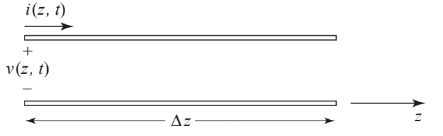
\includegraphics[width=\linewidth]{images/Transmission Line Theory/TransmissionLine-1.png}
        \caption{}
    \end{subfigure}
    \hfill
    \begin{subfigure}{0.48\linewidth}
        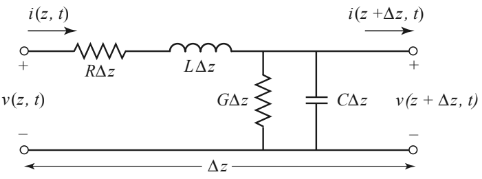
\includegraphics[width=\linewidth]{images/Transmission Line Theory/TransmissionLine-2.png}
        \caption{}
    \end{subfigure}
    \caption{(a) A tranmission line. (b) The equivalent lumped-circuit of the transmission line.}
    \label{fig:Ch1-TransmissionLineCircuit}
\end{figure}
The equations relating the current and voltage of the transmission lines are called the \coltextit{telegrapher equations} and are given in the time-domain as: 
\begin{empheq}[box=\eqnGreenBox]{align}
    \dfrac{\partial}{\partial t} v(z,t) &= -Ri(z,t) - L\dfrac{\partial}{\partial t} i(z,t) \\[2pt] 
    \dfrac{\partial}{\partial t} i(z,t) &= -Gv(z,t) - C\dfrac{\partial}{\partial t} v(z,t)
\end{empheq}
and in the phasor-domain:
\begin{empheq}[box=\eqnGreenBox]{align}
    \dfrac{d}{dz}\phasor{V}(z) &= -(R+j\omega L) \phasor{I}(z) \label{eq:TelegrapherEqn1} \\ 
    \dfrac{d}{dz}\phasor{I}(z) &= -(G+j\omega C) \phasor{V}(z) \label{eq:TelegrapherEqn2}
\end{empheq}

See Proof \ref{der:TelegrapherEquations} for how the telegrapher equations are obtained. 
\begin{proofBox}[Telegrapher Equations] \label{der:TelegrapherEquations}
    By Kirchoff's voltage and current laws, the following equations are obtained: 
    \begin{subequations}
    \begin{align}
        v(z,t) - R \Delta z\ i(z,t) - L \Delta z\ \dfrac{\partial}{\partial t}i(z,t) - v(z+\Delta z, t) &= 0 \\ 
        i(z,t) - G\Delta z \ v(z+\Delta z, t) - C\Delta z\ \dfrac{\partial}{\partial t}v(z+\Delta z, t) - i(z+\Delta z, t) &= 0 
    \end{align}
    \end{subequations}
    By rearranging the terms, the equations can be written as: 
    \begin{subequations}
    \begin{align}
        \dfrac{v(z+\Delta z, t) - v(z,t)}{\Delta z} &= -R i(z,t) - L\dfrac{\partial}{\partial t} i(z,t) \\ 
        \dfrac{i(z+\Delta z, t) - i(z,t)}{\Delta z} &= -Gv(z,t) - C\dfrac{\partial}{\partial t} v(z,t)
    \end{align}
    \end{subequations}
    Finally, by taking the limit as $\Delta z \to 0$ to both sides, we end up with the partial derivatives $\partial v(z,t)/\partial t$ and $\partial i(z,t)/\partial t$ on the left sides; the right sides are unaffected by the limit as there are no $\Delta z$ terms. And finally, we end up with the time-domain representation of the telegrapher equations:
    \begin{subequations}
    \begin{empheq}[box=\fbox]{align}
        \dfrac{\partial}{\partial t} v(z,t) &= -Ri(z,t) - L\dfrac{\partial}{\partial t} i(z,t) \\[2pt] 
        \dfrac{\partial}{\partial t} i(z,t) &= -Gv(z,t) - C\dfrac{\partial}{\partial t} v(z,t)
    \end{empheq}
    \end{subequations}
    Now let's perform the analysis in the phasor-domain. Using Kirchoff's voltage/current laws, we have: 
    \begin{subequations}
    \begin{align}
        \phasor{V}(z) - \phasor{I}(z)R\Delta z - \phasor{I}(z) j\omega L - \phasor{V}(z+\Delta z) &= 0 \\ 
        \phasor{I}(z) - (G\Delta z + j\omega C\Delta z)\phasor{V}(z) - \phasor{I}(z+\Delta z) &= 0
    \end{align}
    \end{subequations}
    Rearranging the equations, 
    \begin{subequations}
        \begin{align}
            \dfrac{\phasor{V}(z+\Delta z) - \phasor{V}(z)}{\Delta z} &= -(R+j\omega L) \phasor{I}(z) \\ 
            \dfrac{\phasor{I}(z+\Delta z) - I(z)}{\Delta z} &= -(G+j\omega C) \phasor{V}(z)
        \end{align}
    \end{subequations}
    And taking the limit as $\Delta z \to 0$, we have the telegrapher equations in the phasor-domain: 
    \begin{subequations}
    \begin{empheq}[box=\fbox]{align}
        \dfrac{d}{dz}\phasor{V}(z) &= -(R+j\omega L) \phasor{I}(z) \\ 
        \dfrac{d}{dz}\phasor{I}(z) &= -(G+j\omega C) \phasor{V}(z)
    \end{empheq}
    \end{subequations}
\end{proofBox}

% *****************************************
% Wave Propagation on a Transmission Line
% *****************************************
\section{Wave Propagation on a Transmission Line}
From solving Eqs.\ (\ref{eq:TelegrapherEqn1}) and (\ref{eq:TelegrapherEqn2}), the wave equations for $\phasor{V}(z)$ and $\phasor{I}(z)$ are obtained: 
\begin{empheq}[box=\eqnGreenBox]{align}
    \dfrac{d^2}{dz^2}\phasor{V}(z) - \gamma^2 \phasor{V}(z) &= 0 \label{eq:WaveEqn1} \\ 
    \dfrac{d^2}{dz^2} \phasor{I}(z) - \gamma^2 \phasor{I}(z) &= 0 \label{eq:WaveEqn2}
\end{empheq}
where $\gamma$ is the complex propagation constant
\begin{equation}
    \gamma = \alpha + j\beta = \sqrt{(R+j\omega L)(G+j\omega C)} \label{eq:PhaseContant}
\end{equation}
$\alpha$ is called the attenuation constant, and $\beta$ is the phase constant. The solution to Eqs. (\ref{eq:WaveEqn1}) and (\ref{eq:WaveEqn2}) is 
\begin{empheq}[box=\eqnGreenBox]{align}
    \phasor{V}(z) &= V_0^+ e^{-\gamma z} + V_{0}^- e^{\gamma z} \label{eq:VoltageEqn} \\ 
    \phasor{I}(z) &= I_0^+e^{-\gamma z} + I_0^- e^{\gamma z} \label{eq:CurrentEqn}
\end{empheq}
where the $e^{-\gamma z}$ term represents wave propagation in the $+z$ direction, and $e^{\gamma z}$ represents wave propagation in the $-z$ direction. The constants $V_0^+$ and $V_0^-$ (or $I_0^+$ and $I_0^-$) are unknown but can be determined if the source and load of the transmission line are known. Note that these constants are complex numbers. 
\begin{subequations}
\begin{align}
    V_0^+ = |V_0^+| e^{j\phi^+} \\ 
    V_0^- = |V_0^-| e^{j\phi^-}
\end{align}
\end{subequations}
%
\begin{note}[The Complex Propagation Constant] \phantom \newline
\begin{itemize}
    \item The propagation constant characterizes how the voltage/current changes along the transmission line.

    \item The attenuation constant tells us how lossy the line is; $\alpha=0$ means the line is lossless whereas $\alpha > 0$ means the line is lossy. The units are Nepres per metre, Np/m.

    \item The phase constant represents the rate at which the phase of the travelling wave along the line varies, and has units of rad/m. 
\end{itemize}
\end{note}
%
The characteristic impedance of the transmission line, $Z_0$, is defined as 
\begin{empheq}[box=\eqnGreenBox]{equation}
    Z_0 = \dfrac{V_0^+}{I_0^+} = \dfrac{-V_0^-}{I_0^-} = \dfrac{R+j\omega L}{\gamma} = \sqrt{\dfrac{R+j\omega L}{G + j\omega C}} \label{eq:CharacteristicImpedance}
\end{empheq}
The current along the transmission line can then be written as 
\begin{equation}
    \phasor{I}(z) = \dfrac{V_0^+}{Z_0} e^{-\gamma z} - \dfrac{V_0^-}{Z_0} e^{\gamma z}
\end{equation}
%
\begin{note}[The Characteristic Impedance $Z_0$] \phantom \newline
\begin{itemize}
    \item The characteristic impedance $Z_0$ is defined as the ratio of the incident voltage to current wave. 
    \item It is not to be confused with the electrical impedance. E.g., if $Z_0 = 50\ \Omega$, this does not mean that the transmission line is equivalent to a lumped $50\ \Omega$ resistor. 
    \item Eq.\ \ref{eq:CharacteristicImpedance} may be used to find the values of the equivlent lumped components of the line. 
\end{itemize}
\end{note}
%
The phase velocity of a wave along a transmission line is 
\begin{equation}
    v_p = \dfrac{\omega}{\beta} = \dfrac{1}{\sqrt{LC}}
\end{equation}
The corresponding wavelength of a wave travelling on the transmission line is then 
\begin{empheq}[box=\eqnGreenBox]{align}
    \lambda_g = \dfrac{v_p}{f} = \dfrac{2\pi}{\beta}
\end{empheq}
$\lambda_g$ is called the guided wavelength. 
%
\begin{note}[Phase Velocity $v_p$ and Guided Wavelength $\lambda_g$] \phantom \newline 
\begin{itemize}
    \item The phase velocity only represents the velocity of the wavefront; that is to say, the velocity of the peaks of a wave for a single frequency/wavelength. The phase velocity may be larger/smaller than the speed of light $c$ depending on the medium. In free-space, $v_p = c$. 
    
    \item The group velocity is the velocity of which the entire wave/particle is travelling at, and this velocity cannot be larger than $c$. The group wave is essentially the sum of all the waves of individual wavelengths/frequencies that are travelling together (recall by the Fourier series that a sinusoidal wave can be expressed as the sum of waves of varying frequencies). If we're looking at just a wave-packet that only consists of one wavelength/frequency, then its phase velocity is equal to the group velocity. 

    \item In electromagnetic texts, you'll see $\lambda$ used by the author to denote either $\lambda_0$ (free-space wavelength) or $\lambda_g$. It is up to you determine the author's notation as one author may use $\lambda$ to refer to the guided wavelength while another will use it to refer to the free-space wavelength. But as a rule of thumb, in the context of transmission lines, $\lambda$ is $\lambda_g$. Otherwise, $\lambda$ is $\lambda_0$. 

    \item Throughout this document, I will explicitly denote the wavelength by $\lambda_g$ or $\lambda_0$ for clarity.
\end{itemize}
\end{note}

% --- Lossless Transmission Lines
\subsection{Lossless Transmission Lines} \label{sec:LosslessLines}
In a lossless transmission line, $R = G = 0$, so Eq. (\ref{eq:PhaseContant}) becomes 
\begin{equation}
    \gamma = \alpha + j\beta = j\omega\sqrt{LC}
\end{equation}
 or
\begin{subequations}
\begin{align}
    \alpha &= 0 \\ 
    \beta &= \omega\sqrt{LC}
\end{align}
\end{subequations}
The wavelength is then 
\begin{equation}
    \lambda_g = \dfrac{2\pi}{\beta} 
\end{equation}
A useful equation for $\beta$ in a lossless line is 
\begin{equation}
    \beta = \omega\sqrt{\mu\varepsilon} = \omega\sqrt{LC}
\end{equation}
where $\mu$ and $\varepsilon$ is the magnetic permeability and electric permittivity, respectively. \par 

The characteristic impedance becomes 
\begin{equation}
    Z_0 = \sqrt{\dfrac{L}{C}} 
\end{equation}
The general solutions for voltage and current become 
\begin{subequations} 
\begin{align}
    \phasor{V}(z) &= V_0^+ e^{-j\beta z} + V_0^- e^{j\beta z} \\ 
    \phasor{I}(z) &= \dfrac{V_0^+}{Z_0} e^{-j\beta z} - \dfrac{V_0^-}{Z_0} e^{j\beta z}
\end{align}
\end{subequations}

% *****************************************
% The Terminated Lossless Transmission Line
% *****************************************
\section{Terminated Transmission Lines} \label{sec:TerminatedLines}
Consider Fig.\ \ref{fig:TL_Load}.

\begin{figure}[!htp]
    \centering
    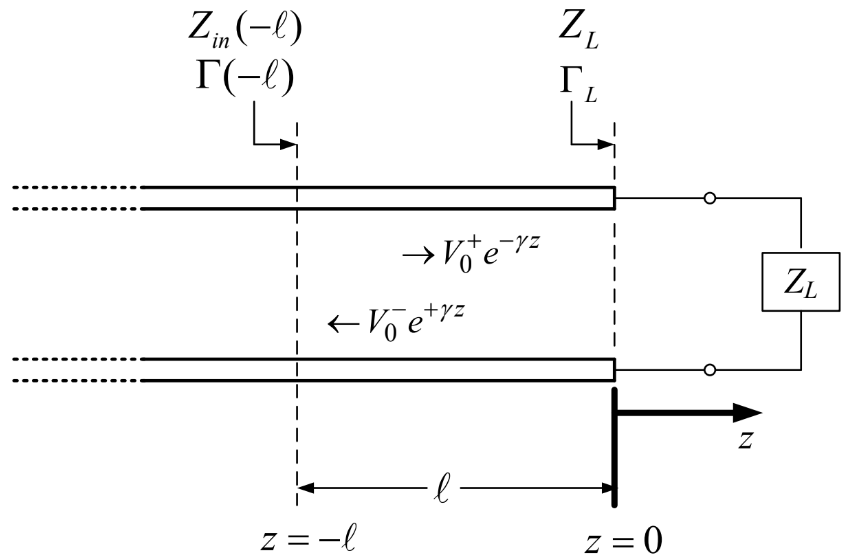
\includegraphics[width=0.7\linewidth]{images/Transmission Line Theory/TL_Load2.png}
    \caption{Transmission line terminated by a load impedance $Z_L$.}
    \label{fig:TL_Load}
\end{figure}

The voltage and current on a transmission line are a superposition of the incident and reflected waves: 
\begin{subequations}
\begin{empheq}[box=\eqnGreenBox]{align}
    \phasor{V}(z) &= V_0^+ e^{-\gamma z} + V_0^- e^{\gamma z} \\ 
    \phasor{I}(z) &= \dfrac{V_0^+}{Z_0} e^{-\gamma z} - \dfrac{V_0^-}{Z_0} e^{\gamma z}
\end{empheq}
\end{subequations}
where $V_0^+$ and $V_0^-$ are complex amplitudes of the incident and reflected waves, respectively. From Fig.\ \ref{fig:TL_Load} we can see that the load impedance is the ratio of the voltage to current at the position $z=0$: 
\begin{equation}
    Z_L = \dfrac{\phasor{V}(0)}{\phasor{I}(0)} = \dfrac{V_0^+ + V_0^-}{V_0^+ - V_0^-} Z_0
\end{equation}
Solving gives 
\begin{empheq}[box=\eqnGreenBox]{equation}
    V_0^- = \dfrac{Z_L - Z_0}{Z_L + Z_0} V_0^+ \label{eq:TLTheory_V0_Reflected}
\end{empheq}
The \coltextit{voltage reflection coefficient} is defined as the ratio of the reflected voltage wave amplitude to the incident voltage wave amplitude. At the load ($z=0$), we denote the reflection coefficient by $\Gamma_L$:
\begin{empheq}[box=\eqnGreenBox]{equation}
    \Gamma_L = \dfrac{V_0^-}{V_0^+} = \dfrac{Z_L - Z_0}{Z_L + Z_0} \label{eq:ReflectionCoefficient}
\end{empheq}
where $\Gamma_L$ is a complex number: $\Gamma_L = |\Gamma_L| e^{j\theta}$. Then, the voltage and current waves on the line may be written as 
\begin{subequations}
\begin{empheq}[box=\eqnGreenBox]{align}
    \phasor{V}(z) &= V_0^+ (e^{-\gamma z} + \Gamma_L e^{\gamma z}) \\ 
    \phasor{I}(z) &= \dfrac{V_0^+}{Z_0} (e^{-\gamma z} - \Gamma_L e^{\gamma z}) 
\end{empheq}
\end{subequations}
It is seen from Eq. (\ref{eq:ReflectionCoefficient}) that the reflection coefficient is zero only if $Z_L = Z_0$. In other words, there is only zero reflection when the load impedance is equal to the characteristic impedance of the line. When $Z_L = Z_0$, we say the load is \textit{matched}. If $Z_L \neq Z_0$, then there is some reflection, and the voltage wave is a superposition of the incident and reflected waves; this is called a \coltextit{standing wave}.  

\begin{note}[Special Load Terminations] When a transmission line is terminated by a matched load, a short circuit, or open circuit, we know what the reflection coefficient will be.
\begin{itemize}
    \item If $Z_L=0$ (short circuit) then $\Gamma_L = -1$ and $|\Gamma_L|=1$.
    \item If $Z_L\to\infty$ (open circuit) then $\Gamma_L$ = 1 and $|\Gamma_L|=1$. 
    \item If $Z_L = Z_0$ (matched load) then $\Gamma_L = 0$. 
    \item If $\Re\{Z_L\} = 0$ (purely reactive load) then $|\Gamma_L|=1$. 
\end{itemize}
\end{note}

An impedance may be normalized to the characteristic impedance. The normalized load impedance $z_L$ is 
\begin{equation}
    z_L = \dfrac{Z_L}{Z_0} = \dfrac{1+\Gamma_L}{1-\Gamma_L}
\end{equation}
A Smith Chart (which is discussed in Section TBD) is an example of where you will see normalized impedances. \par 

At a distance $l$ from the load ($z=-l$), the impedance seen looking towards the load is 
\begin{empheq}[box=\eqnGreenBox]{equation}
    Z_\txtin(-l) = \dfrac{\phasor{V}(-l)}{\phasor{I}(-l)} = Z_0 \left[\dfrac{1+\Gamma_L e^{-2\gamma l}}{1 - \Gamma e^{-2\gamma l}}\right] = Z_0 \left[ \dfrac{Z_L+Z_0\tanh(\gamma l)}{Z_0 + Z_L\tanh(\gamma l)} \right] \label{eq:TLInputImpedance}
\end{empheq}
Similarly, the reflection coefficient at a distance $l$ is 
\begin{empheq}[box=\eqnGreenBox]{equation}
    \Gamma(-l) = \left. \dfrac{V_0^- e^{\gamma z}}{V_0^+ e^{-\gamma z}} \right|_z=-l = \Gamma_L e^{-2\gamma l}
\end{empheq}
The average power on the line can be shown to be 
\begin{empheq}[box=\eqnGreenBox]{equation}
    P_\txtavg = \dfrac{1}{2} \Re\{\phasor{V}(z) \phasor{I}^*(z) \} = \dfrac{1}{2} \dfrac{|V_0^+|^2}{Z_0} (1 - |\Gamma|^2) \label{eq:TLPower}
\end{empheq}
which means that the average power is constant along any point on the line and the total power is equal to the incident minus the reflected. 
\begin{equation}
    P_\txtavg = P_\txtinc - P_\txtrefl
\end{equation}
Note that Eq. (\ref{eq:TLPower}) assumes the generator is matched. \par 

When the load has some mismatch, the load reflects some of the incident power. The loss caused by reflected power is called \coltextit{return loss} (RL). In dB, RL is defined as 
\begin{equation}
    \mathrm{RL}\ [\mathrm{dB}] = -20\log|\Gamma| 
\end{equation}
Recall that we said the waves on the transmission line are standing waves (except when $\Gamma = 0$). So, we define the \coltextit{standing wave ratio} (SWR) which is a ratio of the maximum voltage ampltitude to the minimum amplitude: 
\begin{equation}
    \mathrm{SWR} = \dfrac{V_\txtmax}{V_\txtmin} = \dfrac{1+|\Gamma|}{1-|\Gamma|}
\end{equation}
$\mathrm{SWR}=1$ implies a matched load. 

% --- 
\subsection{Equations for the Lossless Line}
The equations discussed in Section \ref{sec:TerminatedLines} are applicable to lossless transmission lines as well. From Section \ref{sec:LosslessLines}, in a lossless line, $\alpha=0$, which means $\gamma = j\beta$. Therefore, the equations from the previous section remain the same except the following terms are changed: 
\begin{itemize}
    \item $e^{-\gamma l} \longrightarrow e^{-j\beta l}$
    \item $e^{\gamma l} \longrightarrow e^{j\beta l}$
\end{itemize}
For example, we may write the inuput impedance from Eq.\ (\ref{eq:TLInputImpedance}) to be 
\begin{equation}
    Z_\txtin(-l) = \dfrac{\phasor{V}(-l)}{\phasor{I}(-l)} = Z_0 \left[\dfrac{1+\Gamma_L e^{-2j\beta l}}{1 - \Gamma e^{-2j\beta l}}\right] = Z_0 \left[ \dfrac{Z_L+jZ_0\tan(\beta l)}{Z_0 + jZ_L\tan(\beta l)} \right] 
\end{equation}

% *****************************************
% Transmission Line with Load and Source Connected
% *****************************************
\subsection{Transmission Line with Load and Source Connected}

Now a source is connected to a transmission line of length $d$ terminated by a load $Z_L$, as shown in Fig.\ \ref{fig:TLSourceAndLoad}.

\begin{figure}[!htp]
    \centering
    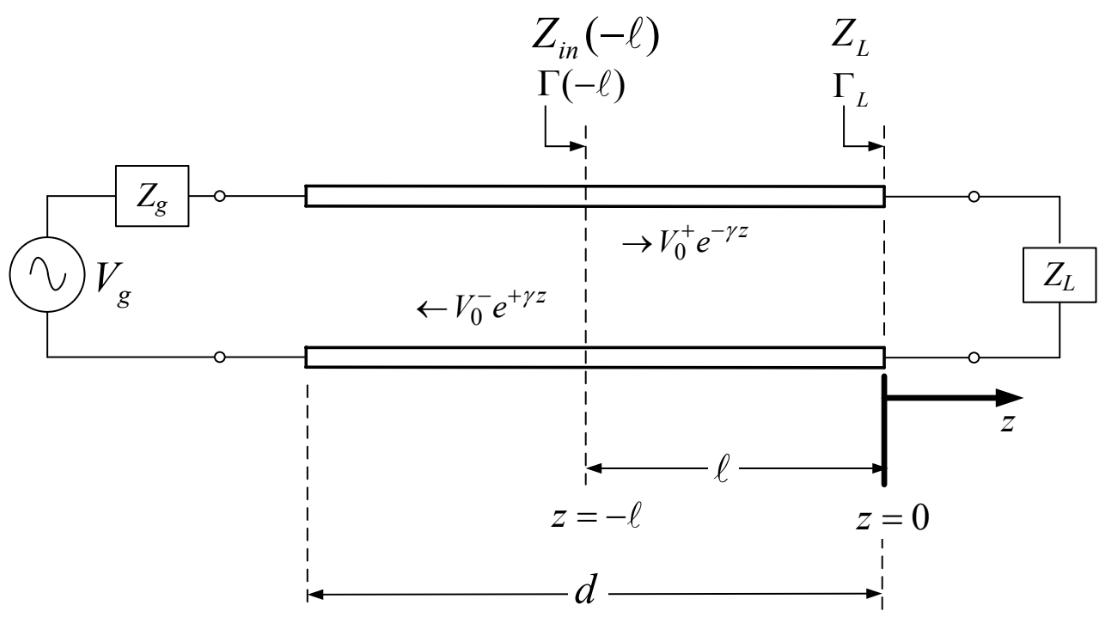
\includegraphics[width=0.8\linewidth]{images/Transmission Line Theory/TL_Source_And_Load.png}
    \caption{Transmission line connected to a source and load.}
    \label{fig:TLSourceAndLoad}
\end{figure}

It can be shown that 
\begin{equation}
    V_0^+ = V_g \left(\dfrac{Z_0}{Z_0+Z_g} \right) \left(\dfrac{e^{-\gamma d}}{1-\Gamma_L\Gamma_G e^{-2\gamma d}} \right)
\end{equation}
where 
\begin{equation}
    \Gamma_G = \dfrac{Z_g - Z_0}{Z_g + Z_0}
\end{equation}
Then, one can find $V_0^-$ by Eqs.\ (\ref{eq:TLTheory_V0_Reflected}), (\ref{eq:ReflectionCoefficient}). The power on the line is 
\begin{equation}
    P_\text{avg}(z) = \dfrac{1}{2} \Re\{\phasor{V}(z) \phasor{I}^*(z) \} = P_i(z) + P_r(z)
\end{equation}
where $P_i(z)$ and $P_r(z)$ denote the incident and reflected power. 
\begin{align}
    P_i(z) &= \dfrac{1}{2} \dfrac{|V_0^+|^2}{Z_0} e^{-2\alpha z} \\ 
    P_r(z) &= \dfrac{1}{2} \dfrac{|V_0^-|^2}{Z_0} e^{2\alpha z}
\end{align}

% *****************************************
% Smith Charts
% *****************************************
\section{Smith Charts}
The Smith chart was invented by P.\ Smith in 1939 and is a graphical tool used to analyze transmission lines. Smith charts are especially useful for impedance matching. \par 

A Smith chart is a polar plot of the complex reflection coefficient with grid lines corresponding to normalized impedances. In Fig.\ \ref{fig:SmithChart2}, we see the basic structure of the Smith chart; the real part of the reflection coefficient ($\Gamma_r$) is along the horizontal axis while the imaginary part ($\Gamma_i$). In Fig.\ \ref{fig:SmithChart_RLXLCircles}, some grid lines corresponding to various impedances are shown on a Smith chart. Fig.\ \ref{fig:SmithChart} shows a typical chart you would use for hand-calculations. \par 

The normalized impedance is represented with a lower-case variable $z$:
\begin{equation}
    z = \dfrac{Z}{Z_0}
\end{equation}
If a lossless transmission line with characteristic impedance $Z_0$ is terminated by a load $Z_L$, the reflection coefficient at the load can be found as 
\begin{equation}
    \Gamma_L = \dfrac{z_L - 1}{z_L + 1} = |\Gamma_L| e^{j\theta}
\end{equation}
where $z_L = Z_L/Z_0$. Or, 
\begin{equation}
    z_L = \dfrac{1+|\Gamma_L|e^{j\theta}}{1-|\Gamma_L|e^{j\theta}}
\end{equation}
The input impedance at a distance $l$ from the load is  
\begin{equation}
    Z_\text{in} = Z_0 \dfrac{1 + \Gamma_L e^{-2j\beta l}}{1 - \Gamma_L e^{-2j\beta l}}
\end{equation}
The normalized input impedance is then 
\begin{equation}
    z_\text{in} = \dfrac{1 + \Gamma_L e^{-2j\beta l}}{1 - \Gamma_L e^{-2j\beta l}}
\end{equation}
A complete rotation around the Smith chart results in a phase change of $2\pi$ in the reflection coefficient, which is equivalent to a

\underline{\textit{Some key points about the Smith chart:
}}
\begin{itemize}
    \item The distance of a point anywhere on the chart to the centre represents the magnitude of the reflection coefficient $\Gamma$. 
    \item The center of the Smith chart ($\Gamma = 0$) corresponds to a matched load (no reflection). Notice how the impedance circle $r_L = 1$ intersects this point. 
    \item The radius of the outermost circle on the chart has a magnitude of 1 ($|\Gamma|=1$). The left and right outermost poitns correspond to the case of short-circuit ($\Gamma=-1$) and open-circuit ($\Gamma=1$). 
    \item In Fig.\ \ref{fig:SmithChart}, you can see 3 scales on the outer perimeter of the circle. The most inner scale represents the phase of the reflection coefficient ($\theta$). The middle scale is the wavelengths towards the load, and the outermost scale is wavelengths towards the generator. 
    \item If you plot a point corresponding to the load impedance, and draw a circle which intersects this point and is centred at the centre of the Smith chart, this is called a SWR circle. The point at which the circle intersects the $\Gamma_r$ axis on the right-hand side is the value of the SWR. Fig.\ \ref{fig:SmithChart_VSWRCircle} illustrates this.
    
\end{itemize}

\underline{\textit{Steps for plotting a reflection coefficient $\Gamma$ on the Smith chart:}}
\begin{enumerate}
    \item Given some $\Gamma_L$ or $Z_L$, first obtain the corresponding normalized impedance $z_L$
    \item Locate the corresponding $r_L$ circle on the Smith chart 
    \item Find the corresponding $x_L$ curve
    \item 
    find where the $r_L$ circle and $x_L$ intersect. Plot your point here. This represents the corresponding reflection coefficient on a Smith chart. 
\end{enumerate}

\begin{figure}[!htp]
    \centering
    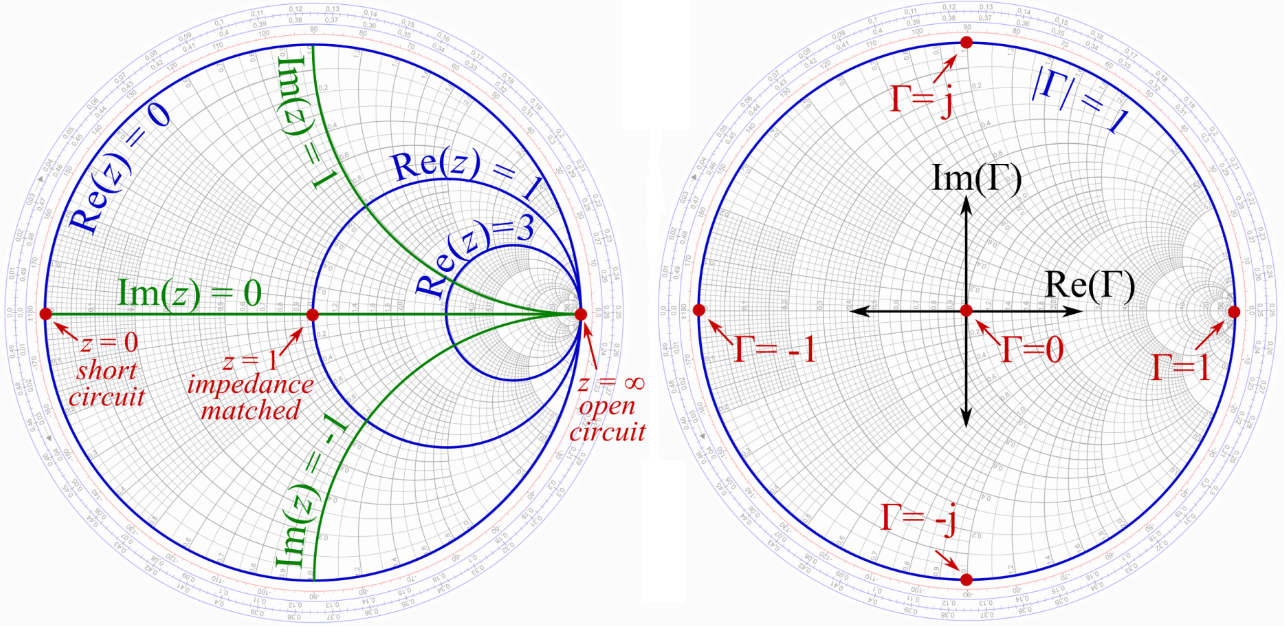
\includegraphics[width=\linewidth]{images/Transmission Line Theory/SmithChart2.png}
    \caption{Smith chart}
    \label{fig:SmithChart2}
\end{figure}

\begin{figure}[!htp]
    \centering
    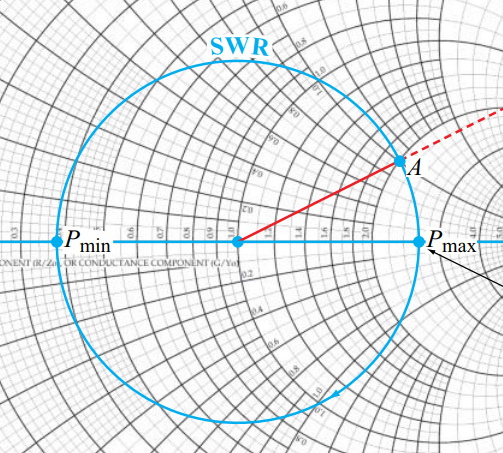
\includegraphics[width=0.5\linewidth]{images/Transmission Line Theory/SmithChart_VSWRCircle.png}
    \caption{VSWR circle on a Smith chart. Point $A$ represents the load impedance. The point $P_\text{max}$ is where the circle intersects the $\Gamma_r$ axis on the right; this is the SWR. In this image, $P_\text{max}$ (and hence SWR) is equal to 2.6.}
    \label{fig:SmithChart_VSWRCircle}
\end{figure}

\begin{figure}[!htp]
    \centering
    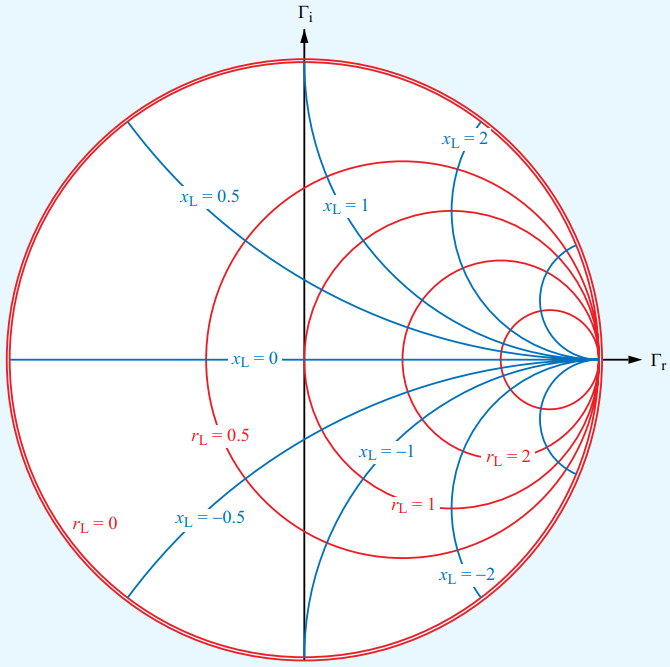
\includegraphics[width=0.5\linewidth]{images/Transmission Line Theory/SmithChart_RLXLCircles.png}
    \caption{Grid lines on a Smith chart corresponding to normalized impedances: $z_L = r_L + j x_L$. }
    \label{fig:SmithChart_RLXLCircles}
\end{figure}

\begin{figure}[!htp]
    \centering
    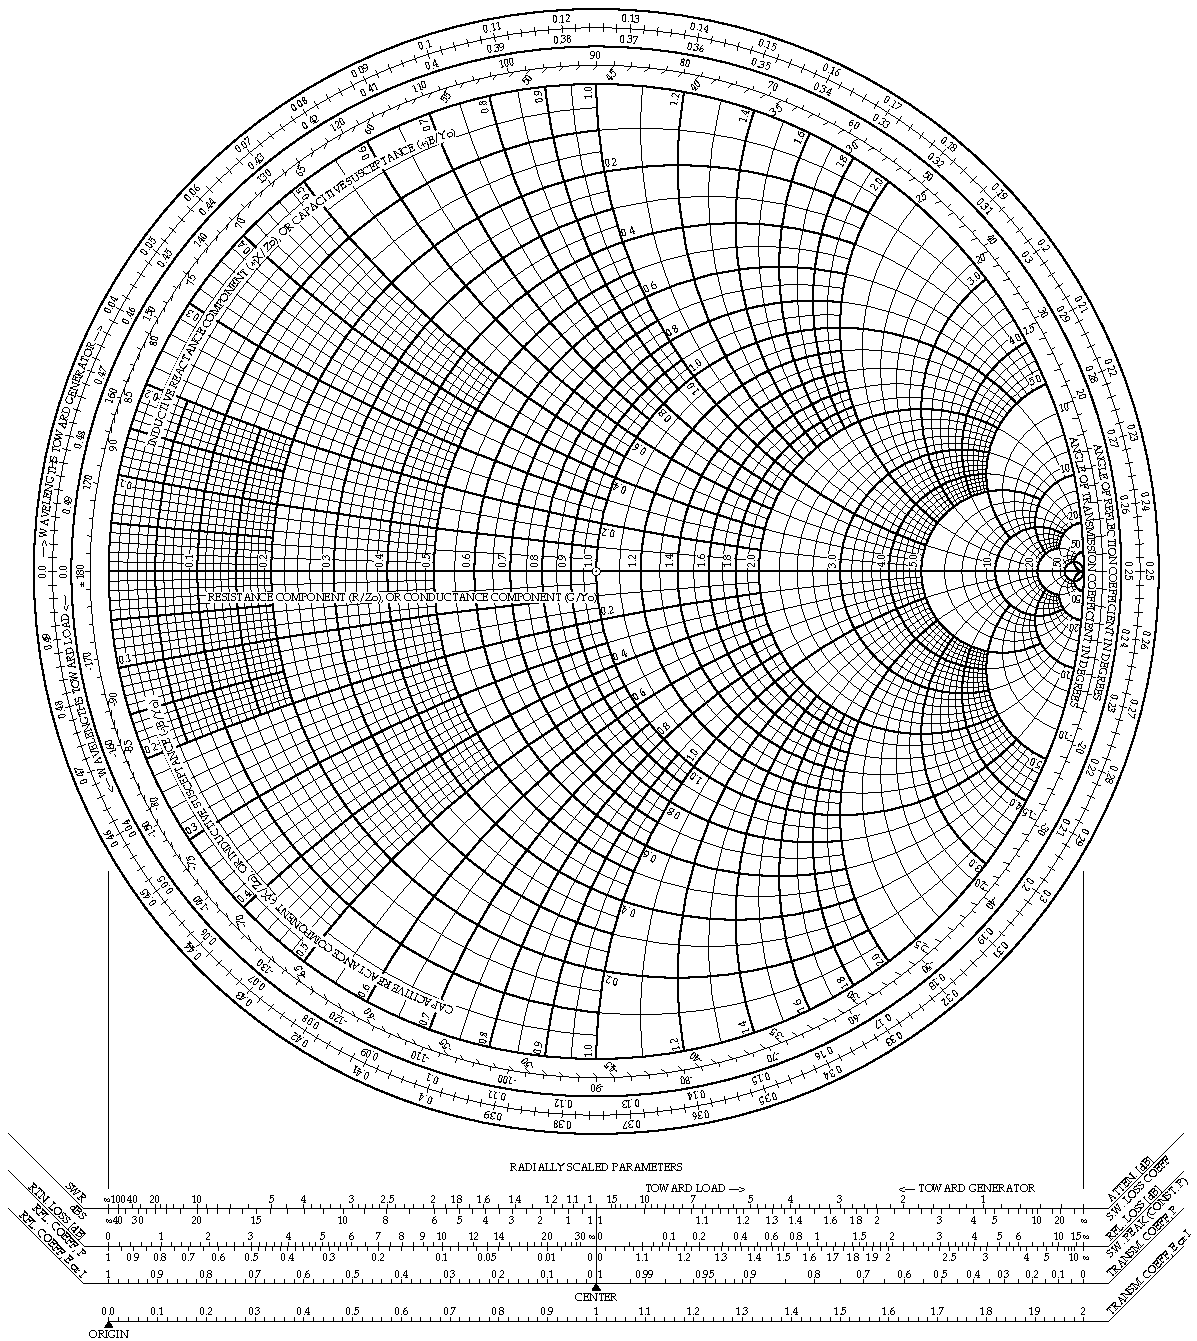
\includegraphics[width=\linewidth]{images/Transmission Line Theory/SmithChart.pdf}
    \caption{The Smith chart}
    \label{fig:SmithChart}
\end{figure}

% Time Varying Fields --------------------------
\chapter{Time-Varying Fields and Maxwell's Equations} \label{ch:TimeVaryingFields}

Maxwell's equations in differential and integral form, in the left and right columns, respectively. 
\begin{empheq}[box=\eqnGreenBox]{align}
    \nabla \cdot \vec{D} &= \rho_v && \oint\limits_S \vec{D} \cdot d\vec{s} = Q \label{eq:Maxwell1}  \\ 
    \nabla \times \vec{E} &= -\dfrac{\partial}{\partial t}\vec{B} && \oint\limits_C \vec{E} \cdot d\vec{l} = -\int\limits_S \dfrac{\partial}{\partial t}\vec{B} \cdot d\vec{s} \label{eq:Maxwell2}   \\ 
    \nabla \cdot \vec{B} &= 0 && \oint\limits_S \vec{B} \cdot d\vec{s} = 0 \label{eq:Maxwell3}   \\ 
    \nabla \times \vec{H} &= \vec{J} + \dfrac{\partial}{\partial t}\vec{D} && \oint\limits_C \vec{H} \cdot d\vec{l} = \int\limits_S \left( \vec{J} + \dfrac{\partial}{\partial t}\vec{D} \right) \cdot d\vec{s} \label{eq:Maxwell4} 
\end{empheq}


% Plane-Wave Propagation -----------------------
\chapter{Plane-Wave Propagation}
In Chapter \ref{ch:TimeVaryingFields}, it was seen that a time-varying electric field $\vec{E}(\vec{r},t)$ produces a time-varying magnetic field $\vec{H}(\vec{r},t)$, and vice versa. Even in the absence of a source excitation, this cyclic pattern often results in an EM wave propagating through free-space or some medium. When a wave propagates in a homogenous medium without interacting with obstacles, it is said to be $\coltextit{unbounded}$. In a lossless medium (like air or a perfect dielectric), the EM wave does not get attenuated. In a lossy medium (material with a non-zero conductivity), the wave does get attenuated and some power is lost as heat. \par 

A source such as an antenna may radiate waves outwardly in the form of a \coltextit{spherical wave}. You can imagine if you drop a rock in a pond, the water waves produces travel outwardly; this is an example of a spherical wave. To an observer standing very far away from the source of a spherical wave, the spherical wave will appear as more ``flat'', as shown in Fig.\ \ref{fig:SphericalWaveFront}. 

\begin{figure}[!htp]
    \centering
    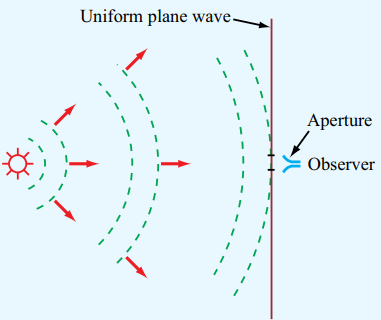
\includegraphics[width=0.3\linewidth]{images/Plane Wave Propagation/SphericalWave.png}
    \caption{Spherical-wave fronts may be approximated as a plane wave if observed at a far distance.}
    \label{fig:SphericalWaveFront}
\end{figure}

To such an observer, the spherical wave may then be approximated as a \coltextit{plane wave}. As the name suggests, a plane wave consists of a plane tangent to the direction of propagation of the wave. The plane wave has identical properties at any point on the plane (e.g. amplitude, phase, polarization, etc.). Fig.\ \ref{fig:PlaneWave} shows a visualization of a plane wave propagating through space. 

\begin{figure}[!htp]
    \centering
    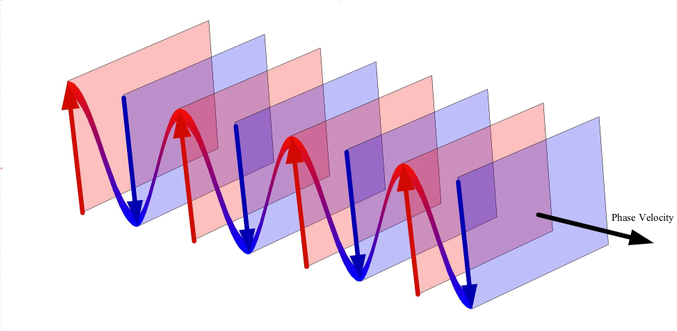
\includegraphics[width=0.5\linewidth]{images/Plane Wave Propagation/PlaneWave.png}
    \caption{Plane wave propagating in space. The red and blue planes represent when the plane wave has a maximum or minimum amplitude, respectively.}
    \label{fig:PlaneWave}
\end{figure}

Plane-waves are good approximations to real waves in many practical situations. For example, in antenna engineering, transmitting and receiving antennas are usually at such far distances from each other that the curvature of the wave fronts are negligible and plane waves may be used for analysis. \par 

When a wave propagates along a material structure, it is said to be travelling in a \coltextit{guided medium} (e.g.\ a transmission line). In Chapter \ref{ch:TransmissionLineTheory} we saw the voltage and current propagation along a transmission line. But, a transmission line can be analyzed with the propagation of electromagnetic waves as well. Thus, we may model wave propagation on a transmission line in terms of voltage and currents along its conductors, or in terms of the electric and magnetic fields in the dielectric medium between the conductors. 

% ===========================================
% Time-Harmonic Fields 
% ===========================================
\section{Time-Harmonic Fields}
Time-varying fields ($\vec{E}, \vec{D}, \vec{H}, \vec{B}$) and their sources ($\rho$, $\vec{J}$) depend on both the position in space and time $t$. But if their variation with time is sinusoidal, the fields and sources may be represented by a \textit{vector phasor} that only depends on the position $\vec{r} = (x,y,z)$. A tilde ($\sim$) will be used to denote vector phasors. For example, relationship between the time-varying field $\vec{E}$ and its corresponding vector phasor $\vecphasor{E}$ is 
\begin{equation}
    \vec{E}(\vec{r}, t) = \Re\{ \vecphasor{E}(\vec{r}) e^{j\omega t} \}
\end{equation}
Maxwell's equations for time-varying fields [Eqs.\ (\ref{eq:Maxwell1})-(\ref{eq:Maxwell4})] may be rewritten in the phasor-domain as 
\begin{align}
    \nabla \cdot \vecphasor{E} &= \dfrac{\phasor{\rho}_v}{\varepsilon} \label{eq:Maxwell_Phasor1} \\ 
    \nabla \times \vecphasor{E} &= -j\omega\mu\vecphasor{H} \label{eq:Maxwell_Phasor2} \\ 
    \nabla \cdot \vecphasor{H} &= 0 \label{eq:Maxwell_Phasor3} \\ 
    \nabla \times \vecphasor{H} &= \vecphasor{J} + j\omega\varepsilon\vecphasor{E} \label{eq:Maxwell_Phasor4}
\end{align}
By defining the \coltextit{complex permittivity} $\varepsilon_c$ as 
\begin{empheq}[box=\eqnGreenBox]{equation}
    \varepsilon_c = \varepsilon - j \dfrac{\sigma}{\omega} = \varepsilon' - j \varepsilon''
\end{empheq}
Maxwell's equations are written as 
\begin{empheq}[box=\eqnGreenBox]{align}
    \nabla \cdot \vecphasor{E} &= 0 \label{eq:Maxwell_Phasor_New1} \\ 
    \nabla \times \vecphasor{E} &= -j\omega\mu\vecphasor{H} \label{eq:Maxwell_Phasor_New2} \\ 
    \nabla \cdot \vecphasor{H} &= 0  \label{eq:Maxwell_Phasor_New3}\\ 
    \nabla \times \vecphasor{H} &= j\omega\varepsilon_c\vecphasor{E} \label{eq:Maxwell_Phasor_New4}
\end{empheq}
More about $\varepsilon_c$ is said later. See Proof \ref{proof:MaxwellEquationsPhasor} for how these were derived. \par 

The \coltextit{wave equations} for $\vecphasor{E}$ and $\vecphasor{H}$ can be shown to be 
\begin{subequations}
\begin{empheq}[box=\eqnGreenBox]{align}
    \nabla^2\vecphasor{E} - \gamma^2\vecphasor{E} &= 0 \label{eq:PlaneWave_WaveEqn1} \\ 
    \nabla^2\vecphasor{H} - \gamma^2\vecphasor{H} &= 0 \label{eq:PlaneWave_WaveEqn2}
\end{empheq}
\end{subequations}
See Proof \ref{proof:WaveEquations} for how the wave equations were derived. 

\begin{proofBox}[Eqs.\ \textcolor{blue-violet}{(\ref{eq:Maxwell_Phasor_New1})-(\ref{eq:Maxwell_Phasor_New4})}] \label{proof:MaxwellEquationsPhasor}
    The conduction current density in a medium with conductivity $\sigma$ is $\vecphasor{J}=\sigma\vecphasor{E}$. Eq.\ (\ref{eq:Maxwell_Phasor4}) may be written as 
    \begin{equation}
        \nabla\times\vecphasor{H} = \vecphasor{J} + j\omega\varepsilon\vecphasor{E} = (\sigma+j\omega\varepsilon)\vecphasor{E} = j\omega\left(\varepsilon-j\dfrac{\sigma}{\omega} \right)\vecphasor{E} = j\omega\varepsilon_c\vecphasor{E}
    \end{equation}
    From vector calculus, the divergence of the curl of any vector field is zero. So, it must be true that $\nabla\cdot\nabla\times\vecphasor{H}=0$. Since we established $\nabla\times\vecphasor{H}=j\omega\varepsilon_c\vecphasor{E}$, we may say 
    \begin{equation}
        \divergence\curl\vecphasor{H} = 0 = \divergence(j\omega\varepsilon_c\vecphasor{E}) \implies \divergence\vecphasor{E} = 0
    \end{equation}
    $\divergence\vecphasor{E}=0$ implies that the charge density $\phasor{\rho}_v = 0$. 
\end{proofBox}

\begin{proofBox}[Wave Equations] \label{proof:WaveEquations}
    Consider Eq.\ (\ref{eq:Maxwell_Phasor_New2}). Taking the curl of both sides, 
    \begin{equation}
        \curl (\curl \vecphasor{E}) = -j\omega\mu(\curl\vecphasor{H})
    \end{equation}
    Substituting Eq.\ (\ref{eq:Maxwell_Phasor_New4}) into this, 
    \begin{equation}
        \curl (\curl\vecphasor{E}) = -j\omega\mu(j\omega\varepsilon_c\vecphasor{E}) = \omega^2\mu\varepsilon_c\vecphasor{E} \label{eq:placeholder1}
    \end{equation}
    Using the identity of a curl of a curl of a field, from vector calculus, 
    \begin{equation}
        \curl(\curl\vecphasor{E}) = \nabla(\divergence\vecphasor{E}) - \nabla^2\vecphasor{E} \label{eq:placeholder2}
    \end{equation}
    where $\nabla^2\vecphasor{E}$ is the Laplacian of $\vecphasor{E}$. By Eq.\ \ref{eq:Maxwell_Phasor_New1}, $\divergence\vecphasor{E}=0$. Now, with Eqs.\ (\ref{eq:placeholder1}) and (\ref{eq:placeholder2}), this gives
    \begin{equation}
        \nabla^2\vecphasor{E} + \omega^2\mu\varepsilon_c\vecphasor{E} = 0
    \end{equation}
    The propagation constant $\gamma$ has the relationship 
    \begin{equation}
        \gamma^2 = -\omega^2\mu\varepsilon_c
    \end{equation}
    Therefore, we are left with 
    \begin{equation}
        \nabla^2\vecphasor{E} - \gamma^2\vecphasor{E} = 0
    \end{equation}
    Similar steps are required with Eq.\ \ref{eq:Maxwell_Phasor_New4} to obtain the wave equation for $\vecphasor{H}$. 
\end{proofBox}

% ===========================================
% Plane-Wave Propagation in Lossless Media
% ===========================================
\section{Plane-Wave Propagation in Lossless Media}
If the medium is nonconducting ($\sigma=0$), the medium is lossless and the wave does not suffer any attenuation. In a lossless medium, $\varepsilon_c = \varepsilon$. 
\begin{equation}
    \gamma^2 = -\omega^2\mu\varepsilon
\end{equation}
The phase velocity is 
\begin{empheq}[box=\eqnGreenBox]{equation}
    v_p = \dfrac{\omega}{k} = \dfrac{1}{\sqrt{\mu\varepsilon}}
\end{empheq}
The wavenumber is
\begin{empheq}[box=\eqnGreenBox]{equation}
    k = \dfrac{2\pi}{\lambda_g} = \omega \sqrt{\mu\varepsilon}
\end{empheq}
In lossless media, $\gamma = jk$. So, the wave equations become
\begin{align}
    \nabla^2 \vecphasor{E} + k^2 \vecphasor{E} &= 0 \\ 
    \nabla^2 \vecphasor{H} + k^2 \vecphasor{H} &= 0
\end{align}
In \cite{Ulaby_textbook} beginning on page 17, it is shown that for a plane wave, there are no electric or magnetic field components in the direction of propagation ($E_z = H_z = 0$). \par 

The \coltextit{intrinsic impedance} in a lossless medium is 
\begin{empheq}[box=\eqnGreenBox]{equation}
    \eta = \dfrac{\omega\mu}{k} = \sqrt{\dfrac{\mu}{\varepsilon}} \qquad [\Omega]
\end{empheq}
In free space, 
\begin{equation}
    \eta_0 = \sqrt{\dfrac{\mu_0}{\varepsilon_0}} = 377\ \Omega \approx 120\pi \ \Omega 
\end{equation}

\begin{note}[Intrinsic impedance, $\eta$]
    The intrinsic wave impedance can also be defined as the magnitude of the E-field component to the H-field component. For example, if $\vecphasor{E}=\uvec{x} E_x$ and $\vecphasor{H}=\uvec{y}H_y$, then 
    \begin{equation}
        \eta = \dfrac{E_x}{H_y}
    \end{equation}
    This is analagous to how we defined the characteristic impedance in Chapter \ref{ch:TransmissionLineTheory}. 
    \begin{equation}
        Z_0 = \dfrac{\phasor{V}}{\phasor{I}}
    \end{equation}
    Note that similar to the characteristic impedance, the intrinsic impedance is not the same as an electric impedance of a resistor. It's simply a ratio of the electric and magnetic fields (or permittivity and permeability) in a given medium. 
\end{note}
For a plane wave travelling in some direction $\uvec{k}$, the electric and magnetic fields are related by 
\begin{empheq}[box=\eqnGreenBox]{align}
    \vecphasor{H} &= \dfrac{1}{\eta} \ \uvec{k} \times \vecphasor{E} \label{eq:E_H_Relation1} \\ 
    \vecphasor{E} &= -\eta \ \uvec{k} \times \vecphasor{H} \label{eq:E_H_Relation2}
\end{empheq}
In many textbooks, such as in Chapter 7 in \cite{Ulaby_textbook}, this general relation can be proved for a plane wave travelling in a direction $\uvec{z}$. A simple antenna engineering-centric proof is given in \ref{proof:GeneralRelation_E_H} to prove this relation for any wave that only has components transverse to the direction of propagation. \par 

The \coltextit{wave impedance} seen by a wave travelling in a direction $\uvec{k}$ is 
\begin{empheq}[box=\eqnGreenBox]{equation}
    Z_w = \dfrac{\uvec{k} \cdot (\vecphasor{E}\times\vecphasor{H}^*)}{(\uvec{k}\times\vecphasor{H}) \cdot (\uvec{k}\times\vecphasor{H}^*)}
\end{empheq}
In free-space, $Z_w = \eta_0$. 

\begin{proofBox}[Relation between $\vecphasor{E}$ and $\vecphasor{H}$] \label{proof:GeneralRelation_E_H}
    This proof takes an antenna engineering-centric approach. Consider the general form of a magnetic field in spherical coordinates.
    $$ \vecphasor{H} = \vecphasor{H}(r,\theta,\phi) = \uvec{r}\ H_r(r,\theta,\phi)  + \uvec{\theta}\ H_\theta(r,\theta,\phi)  + \uvec{\phi}\ H_\phi(r,\theta,\phi)  $$
    Because the magnetic field only has transverse components to the direction of propagation $\uvec{r}$, $H_r = 0$. If we also assume the electromagnetic wave is in far-field relative to its source, the wave can be approximated as a plane wave. Then, $H_\theta$ and $H_\phi$ take the form, 
    \begin{align*}
        H_\theta  &= F_\theta(\theta,\phi) \dfrac{e^{-jkr}}{r} \\
         H_\phi  &= F_\phi(\theta,\phi) \dfrac{e^{-jkr}}{r}
    \end{align*}
    These equations come from antenna engineering texts, such as \cite{Balanis-2012-antenna}. \par 
    %
    Performing the curl of $\vecphasor{H}$, 
    \begin{align*}
        \nabla \times \vecphasor{H} &= 
        \begin{vmatrix}
            \uvec{r}/r^2\sin\theta & \uvec{\theta}/r\sin\theta & \uvec{\phi}/r \\ 
            \partial/\partial r & \partial/\partial \theta & \partial/\partial \phi \\ 
            0 & r H_\theta & r \sin\theta H_\phi
        \end{vmatrix} \\ 
        &= \uvec{r} \ 0 - \dfrac{\uvec{\theta}}{r\sin\theta}\dfrac{\partial}{\partial r} (r\sin\theta H_\phi) + \dfrac{\uvec{\phi}}{r} \dfrac{\partial}{\partial r}(r H_\theta) \\
        &=  - \dfrac{\uvec{\theta}}{r\sin\theta}\dfrac{\partial}{\partial r} \left(r\sin\theta F_\phi \dfrac{e^{-jkr}}{r}\right) + \dfrac{\uvec{\phi}}{r} \dfrac{\partial}{\partial r}\left(r F_\phi \dfrac{e^{-jkr}}{r} \right) \\ 
        &= - \uvec{\theta} \ \dfrac{F_\phi}{r} (-jk) e^{-jkr} + \uvec{\phi} \ \dfrac{F_\theta}{r} (-jk) e^{-jkr} \\ 
        &= \uvec{\theta}\ jk \underbrace{\dfrac{F_\phi e^{-jkr}}{r}}_{H_\phi} + \uvec{\phi} \ jk \underbrace{\dfrac{-F_\theta e^{-jkr}}{r}}_{-H_\theta} 
    \end{align*}
     Using Maxwell's curl equation, 
        $$\nabla \times \vecphasor{H} = j\omega\varepsilon_0\vecphasor{E} = j\omega\varepsilon_0[\uvec{\theta}\ E_\theta + \uvec{\phi}\ E_\phi]$$ 
        a relationship between $\vecphasor{H}$ and $\vecphasor{E}$ can be observed. Note that it is assumed $E_r = 0$ because the electromagnetic fields only have transverse components. So, we have 
        \begin{align*}
           j\omega\varepsilon_0 E_\theta &= jk H_\phi \\ 
            E_\theta &= \dfrac{k}{\omega \varepsilon_0} H_\phi = \dfrac{\omega\sqrt{\mu_0\varepsilon_0}}{\omega \varepsilon_0} H_\phi = \dfrac{\sqrt{\mu_0}}{\sqrt{\varepsilon_0}} H_\phi \\ 
            E_\theta  &= \eta H_\phi \\ 
            \Aboxed{H_\phi &= \eta^{-1} E_\theta} \\
            \intertext{and}
            j\omega\varepsilon_0 E_\phi &= -jk H_\theta \\
            E_\phi &= -\eta H_\theta  \\ 
            \Aboxed{H_\theta  &= -\eta^{-1} E_\phi}
        \end{align*}
        %
        Putting this together,
        \begin{align*}
            \vecphasor{H}(\vec{r}) &= \eta^{-1} [-\uvec{\theta} \ E_\phi + \uvec{\phi} \ E_\theta] \\ 
            &= \eta^{-1} [(\uvec{r}\times\uvec{\phi}) \ E_\phi + (\uvec{r} \times\uvec{\theta}) \ E_\theta] \\ 
            &= \eta^{-1} \ \uvec{r} \times [\uvec{\theta}\ E_\theta + \uvec{\phi}\ E_\phi ] \\
            \Aboxed{\vecphasor{H}(\vec{r}) &= \eta^{-1} \ \uvec{r} \times \vecphasor{E}(\vec{r}) }
        \end{align*}
        With some vector algebra, this may be written as 
        \begin{align*}
            \Aboxed{
            \vecphasor{E}(\vec{r}) &= -\eta \ \uvec{r} \times \vecphasor{H}}
        \end{align*}
        The direction $\uvec{r}$ is just some arbitrary direction (like $\uvec{k}$), so they are interchangeable here, and the same equations as in (\ref{eq:E_H_Relation1}) and (\ref{eq:E_H_Relation2}) are derived. 
\end{proofBox}

% --- General Form of EM Plane Wave 
\subsection{General Form of a Electric and Magnetic Field}
In lossless media, the electric field takes the form 
\begin{empheq}[box=\eqnGreenBox]{equation}
    \vecphasor{E}(z) = \uvec{x} \ \phasor{E}_x(z) + \uvec{y}\ \phasor{E}_y(z)
\end{empheq}
where 
\begin{align}
    \phasor{E}_x(z) &= E_{x_0} e^{-jkz} \\ 
    \phasor{E}_y(z) &= E_{y_0} e^{-jkz}
\end{align}
where $E_{x_0}$ and $E_{y_0}$ are amplitudes and are complex numbers. By Eq.\ (\ref{eq:E_H_Relation1}), an expression for the magnetic field can be obtained. With $\uvec{k} = \uvec{z}$, $\uvec{z} \times \uvec{x} = \uvec{y}$ and $\uvec{z} \times \uvec{y} = -\uvec{x}$, 
\begin{equation}
    \vecphasor{H}(z) = - \uvec{x} \ \dfrac{\phasor{E}_y}{\eta} + \uvec{y} \ \dfrac{\phasor{E}_x}{\eta}
\end{equation}

% ===========================================
% Polarization
% ===========================================
\section{Polarization}
Polarization refers to how the phasor form of the electric field changes over time. The polarization of a wave can be determined by the phase difference between the components of the field. The amplitudes of the $x$ and $y$ components of the electric field are %
\begin{subequations} %
\begin{align}
    E_{x_0} &= a_x \\ 
    E_{y_0} &= a_y e^{j\delta}
\end{align}
\end{subequations}
where $a_x$ and $a_y$ are constants, and $\delta$ is the phase difference between the components. Here, the absolute phase of each component is not important; the relative phase $\delta$ is what matters. In the phasor-domain, the components of the electric field are then 
\begin{align}
    \phasor{E}_x(z) &= a_x e^{-jkz} \\ 
    \phasor{E}_y(z) &= a_y e^{j\delta} e^{-jkz}
\end{align}
In the time-domain, this translates to 
\begin{align}
    E_x(t,z) &= a_x \cos(\omega t - kz) \\
    E_y(t,z) &= a_y \cos(\omega t - kz + \delta) 
\end{align}
And the field is 
\begin{align}
    \vec{E}(t,z) = \uvec{x} \ a_x \cos(\omega t - kz) + \uvec{y}\ a_y \cos(\omega t - kz + \delta) 
\end{align}
If we were to fix the position and just observe the field with respect to time, 
\begin{equation}
    \vec{E}(t) = \uvec{x}\ a_x \cos(\omega t) + \uvec{y}\ a_y \cos(\omega t + \delta) 
\end{equation}
The magnitude of the electric field is 
\begin{equation}
    |\vec{E}(t)| = \sqrt{E_x^2(t) + E_y^2(t)}
\end{equation}
and the orientation of the field in the $xy$-plane (perpendicular to the direction of propagation) over time is 
\begin{equation}
    \alpha(t) = \arctan\left(\dfrac{E_y(t)}{E_x(t)} \right)
\end{equation}
Let's consider three special cases: linear, circular, and elliptical polarization. 

% --- Linear Polarization 
\subsection{Linear Polarization} 
Linear polarization (LP) occurs $E_x(t)$ and $E_y(t)$ are in phase ($\delta=0$) or out of phase ($\delta=\pi$). In both cases, the field magnitude is
\begin{align}
    |\vec{E}(t)| = \sqrt{E_x^2(t) + E_y^2(t)} = \sqrt{a_x^2 + a_y^2} \cos(\omega t)
\end{align}
(when $\delta=\psi$, $\cos(\omega t \pm 180) = -\cos(\omega t)$). Depending on whether the field components are in phase or out of phase, the orientation $\alpha(t)$ differs: 
\begin{subequations}
\begin{align}
    \alpha(t) &= \arctan\left(\dfrac{a_y}{a_x} \right) && \text{(in phase)} \\ 
    \alpha(t) &= \arctan\left(\dfrac{-a_y}{a_x} \right) && \text{(out of phase)}
\end{align}
\end{subequations}
It is seen that the orientation does not differ with time for LP.

\begin{figure}[!htp]
    \centering
    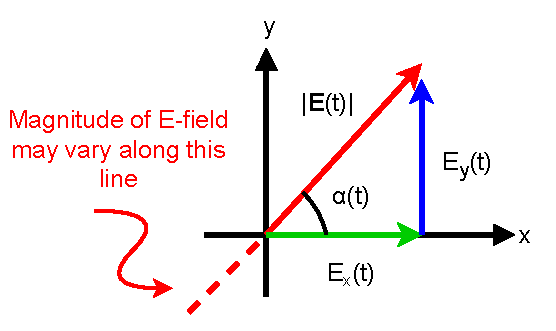
\includegraphics[width=0.6\linewidth]{images/Plane Wave Propagation/LinearPolarization.pdf}
    \caption{Linear polarization. The magnitude of the E-field may oscillate along the solid/dashed red line.}
    \label{fig:LinearPolarization}
\end{figure}

% Example 
\begin{example}
    The electric field of a plane wave is given by 
    $$ \vec{E}(z,t) = \uvec{x}\ 3\cos(\omega t - kz) + \uvec{y}\ 4\cos(\omega t - kz) $$
    Determine the (a) polarization state, (b) modulus of $\vec{E}$, and (c) orientation angle $\alpha$

    \vspace{0.25cm}
    \textbf{Solution:} 
    \begin{enumerate}[label=(\alph*)]
        \item The phase of the $x$ and $y$ components are zero ($\phi_x = \phi_y = 0$) and the phase difference is thus $\delta_s = 0$. Therefore, this plane wave is linearly polarized (LP).  

        \item The modulus $|\vec{E}|$ is 
        \begin{align*}
            |\vec{E}| &= \sqrt{E_x^2 + E_y^2} \\ 
            &= \sqrt{[3\cos(\omega t - kz)]^2 + [4\cos(\omega t - kz)]^2} \\ 
            &= \cos(\omega t - kz) \sqrt{9 + 16} \\ 
            &= 5 \cos(\omega t - kz) \qquad [\text{V/m}]
        \end{align*}

        \item The orientation angle is 
        \begin{align*}
            \alpha &= \arctan\left(\dfrac{E_y}{E_x}\right) = \arctan\left(\dfrac{4\cos(\omega t - kz)}{3\cos(\omega t - kz)} \right) = \arctan\left(\dfrac{4}{3} \right) \\ 
            &= 53.1\degree
        \end{align*}
    \end{enumerate}
\end{example}

% --- Circular Polarization 
\subsection{Circular Polarization}
For circular polarization, the magnitudes of the field components are equal ($a_x = a_y$) and the phase difference is $\delta = \pm\pi/2$. When $\delta=\pi/2$, it is called \coltextit{left-hand circular} polarization (LHCP) and when $\delta = -\pi/2$, it is called \coltextit{right-hand circular} polarization (RHCP). With LHCP, $\alpha(t)$ rotates CW, and with RHCP, $\alpha(t)$ rotates CCW with time. \par 

For both LHCP and RHCP, let's set the constants to the same value: $a_x = a_y = a$. One component will have a term with $\cos(\omega t)$ while the other will have a term with $\cos(\omega t \pm \pi/2) = \mp \sin(\omega t)$. For both cases, the magnitude turns out to be $a$: 
\begin{align}
    |\vec{E}(t)| = \sqrt{E_x^2(t) + E_y^2(t)} = \sqrt{a^2\cos^2(\omega t) + a^2\sin^2(\omega t)} = a 
\end{align}

\underline{\large \textsl{LHCP}} \\[0.25cm] 
In this case, $E_x(t) = a\cos(\omega t)$ and $E_y(t) = -a\sin(\omega t)$. The orientation over time comes out to be 
\begin{equation}
    \alpha(t) = \arctan\left(\dfrac{E_y(t)}{E_x(t)}\right) = \arctan\left(\dfrac{-a\sin(\omega t)}{a\cos\omega t} \right) = -\omega t
\end{equation}

\vspace{0.5cm}

\underline{\large \textsl{RHCP}} \\[0.25cm] 
Now, $E_x(t) = a\cos(\omega t)$ and $E_y(t) = a\sin(\omega t)$. The orientation is 
\begin{equation}
    \alpha(t) = \omega t
\end{equation}

\begin{figure}[!htp]
    \centering
    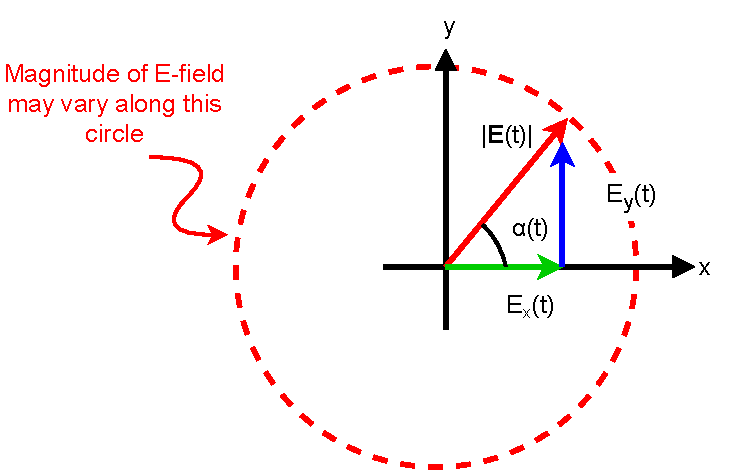
\includegraphics[width=0.7\linewidth]{images/Plane Wave Propagation/CircularPolarization.pdf}
    \caption{Circular polarization. The magnitude of the E-field may vary over the dashed circular path. If LHCP, then the vector rotates CW. If RHCP, then CCW.}
    \label{fig:CircularPolarization}
\end{figure}

% --- Elliptical Polarization 
\subsection{Elliptical Polarization}
If a wave is not linearly or circularly polarized, it is elliptically polarized. If $\delta < 0$, we have right-hand elliptical polarization, and if $\delta > 0$, it is left-hand. 

\begin{example}
    Determine the polarization state of a plane wave with electric field 
    $$ \vec{E}(z,t) = \uvec{x}\ 3\cos(\omega t - kz + 30\degree) - \uvec{y}\ 4\sin(\omega t - kz + 45\degree) $$ 

    \vspace{0.25cm}
    \textbf{Solution:} First, convert the second term to a cosine function so that it matches the first term and we can easily examine the phase difference. 
    \begin{align*}
        \vec{E} &= \uvec{x}\ 3\cos(\omega t - kz + 30\degree) - \uvec{y}\ 4\cos(\omega t - kz + 45\degree - 90\degree) \\ 
        &= \uvec{x}\ 3\cos(\omega t - kz + 30\degree) - \uvec{y}\ 4\cos(\omega t - kz - 45\degree) \\ 
        \intertext{Notice the $-\uvec{y}$. We turn this into a $+\uvec{y}$ and add 180$\degree$ of phase. }
        &= \uvec{x}\ 3\cos(\omega t - kz + 30\degree) + \uvec{y}\ 4\cos(\omega t - kz - 45\degree + 180\degree) \\ 
        &= \uvec{x}\ 3\cos(\omega t - kz + 30\degree) + \uvec{y}\ 4\cos(\omega t - kz + 135 \degree)
    \end{align*}
    We see there is a phase difference of $\delta = 135\degree - 30\degree = 105\degree$. Clearly the wave is not LP (because $\delta \neq 0$ or $180\degree$) and not CP (because $\delta \neq \pm 90\degree$). Therefore, this electric field is elliptically polarized, specifically left-handed because $\delta > 0$. 
\end{example}

% ===========================================
% Plane-Wave Propagation in Lossy Media
% ===========================================
\section{Plane-Wave Propagation in Lossy Media}

Recall the propagation constant is defined as
\begin{align}
    \gamma^2 &= -\omega^2\mu\varepsilon_c = -\omega^2\mu(\varepsilon'-j\varepsilon'') \\ 
    \gamma &= \alpha + j\beta 
\end{align}
By solving for $\alpha$ and $\beta$ by substituting these equations into the wave equation (\ref{eq:PlaneWave_WaveEqn1}), we obtain 
\begin{subequations}
\begin{empheq}[box=\eqnGreenBox]{align}
    \alpha &= \omega \left[ \dfrac{\mu\varepsilon'}{2} \left[ \sqrt{1 + \left(\dfrac{\varepsilon''}{\varepsilon'}\right)^2} -1 \right] \right]^{1/2} \qquad [\text{Np/m}] \\ 
    \beta &= \omega \left[ \dfrac{\mu\varepsilon'}{2} \left[ \sqrt{1 + \left(\dfrac{\varepsilon''}{\varepsilon'}\right)^2} + 1 \right] \right]^{1/2} \qquad [\text{rad/m}]
\end{empheq}
\end{subequations}
The intrinsic impedance of a lossy medium is 
\begin{empheq}[box=\eqnGreenBox]{align}
    \eta_c = \sqrt{\dfrac{\mu}{\varepsilon_c}} = \sqrt{\dfrac{\mu}{\varepsilon'}} \left(1 - j\dfrac{\varepsilon''}{\varepsilon'} \right)^{-1/2} \qquad [\Omega]
\end{empheq}
The distance $\delta_s$ is called the \coltextit{skin depth} and characterizes how depp an EM wave can penetrate into a conducting medium: 
\begin{empheq}[box=\eqnGreenBox]{align}
    \delta_s &= \dfrac{1}{\alpha} 
\end{empheq}
As a wave travels through a distance $z=\delta_s$, the wave magnitude decreases by a factor $e^{-1} \approx 0.37$. When $z=3\delta_s$, the magnitude is less than 5\% of its initial value. At $5\delta_s$, it is less than 1\%. \par 
Some key points about skin depth and its relation to good conductors:
\begin{itemize}
    \item In a perfect dielectric, $\sigma=0,\ \varepsilon''=0,\ \alpha=0$, thus $\delta_s=\infty$

    \item In a perfect conductor, $\sigma=\infty,\ \alpha=\infty$, thus $\delta_s = 0$. This means all incident EM waves are reflected. 

    \item For a lossy medium, the ratio $\varepsilon''/\varepsilon'$ that appears in the equations is very important. 

    \item When $\varepsilon''/\varepsilon' \ll 1$, the medium is considered to be a low-loss dielectric. 

    \item When $\varepsilon''/\varepsilon' \gg 1$, the medium is considered a good conductor. 

    \item $\varepsilon''/\varepsilon' = \sigma/(\omega\varepsilon_r\varepsilon_0)$
\end{itemize}

In a good conductor, we may approximate equations for $\alpha,\ \beta,$ and $\eta_c$ to be in a much simpler form: 
\begin{subequations}
\begin{align}
    \alpha &\approx \omega\sqrt{\dfrac{\mu\varepsilon''}{2}} = \sqrt{\pi f\mu\sigma} \\ 
    \beta &= \alpha \approx \sqrt{\pi f \mu\sigma} \\ 
    \eta_c &\approx \sqrt{j\dfrac{\mu}{\varepsilon''}} = (1+j)\sqrt{\dfrac{\pi f\mu}{\sigma}} = (1+j) \dfrac{\alpha}{\sigma}
\end{align}
\end{subequations}

\begin{example}
    A plane wave is travelling in sea water in the $+z$ direction. The constitutive parameters of sea water are $\varepsilon_r=80$, $\mu_r=1$, and $\sigma=4$ S/m. At $z=0$, the electric field is 
    \begin{align*}
        \vec{E}(t) = \uvec{x} 100\cos(10^7 \pi t)
    \end{align*}
    \begin{enumerate}[label=(\alph*), itemsep=0pt]
        \item Determine $\alpha,\ \beta,\ \eta_c,\ v_p,\ \lambda_n$ and $\delta_s$. 
        \item Find the distance at which the amplitude of the E-field is 1\% of its value at $z=0$. 
        \item Write the expressions for $\vec{E}$ and $\vec{H}$ at $z=0.8$ m as a function of time. 
    \end{enumerate}
    \textbf{Solution.} 
    \begin{enumerate}[label=(\alph*), itemsep=0pt]
        \item The angular frequency is $10^7 \pi$. Then, 
            \begin{align*}
                \dfrac{\varepsilon''}{\varepsilon'} &= \dfrac{\sigma}{\omega\varepsilon_r\varepsilon_0} = \dfrac{4}{10^7\pi \times 80 \times 8.85\times10^{-12}} \approx 180 \gg 1 
            \end{align*}
            So, sea water is a good conductor at this frequency. We may use the approximation for a good conductor with the frequency being $f=\omega/2\pi = 5$ MHz. 
            \begin{align*}
                \alpha &= \sqrt{\pi f \mu \sigma} = \sqrt{\pi \cdot (5\times10^6) \cdot (1\times 4\pi\times10^{-7}) \cdot 4} = 8.89 \text{ Np/m} \\ 
                \beta &= \alpha = 8.89 \text{ rad/m} \\ 
                \eta_c &= (1+j)\dfrac{\alpha}{\sigma} = (1+j) \dfrac{8.89}{4} = 2.22(1+j) = 2.22 e^{j\pi/4} \ \Omega \\ 
                \lambda_n &= \dfrac{2\pi}{k} = \dfrac{2\pi}{\beta} = 0.71 \ \text{m}  \\ 
                v_p &= \dfrac{\omega}{k} = \dfrac{\omega}{\beta} = \dfrac{10^7 \pi}{8.89} = 3.53 \times 10^{6} \ \text{m/s} \\ 
                \delta_s &= \dfrac{1}{\alpha} = \dfrac{1}{8.89} = 0.112\ \text{m} 
            \end{align*}

        \item The $x$-component of the electric field in lossy media takes the form 
        \begin{equation*}
            \phasor{E}_x(z) = E_{x_0} e^{-\gamma z} = \underbrace{|E_{x_0}| e^{-\alpha z}}_{\text{amplitude}} e^{-jkz}
        \end{equation*}
        where $|E_{x_0}| e^{-\alpha z}$ is the amplitude. Converting this to the time-domain, 
        \begin{equation*}
            \vec{E}(t,z) = \uvec{x}\ E_x(z) = |E_{x_0}| e^{-\alpha z} \cos(\omega t - kz)
        \end{equation*}
        At $z=0$, the amplitude is 100, which means $|E_{x_0}| e^{-\alpha \cdot 0} = |E_{x_0}| = 100$. So, we would like to find when $|E_{x_0}| e^{-\alpha z}/|E_{x_0}| = 1\% = 0.01 \implies e^{-\alpha z} = 0.01$. 
        \begin{align*}
            e^{-\alpha z} &= 0.01 \\ 
            -\alpha z &= \ln(0.01) \\ 
            z &= -\dfrac{\ln(0.01)}{\alpha} = -\dfrac{\ln(0.01)}{8.89} \\ 
            \Aboxed{z &= 0.52 \ \text{m}}
        \end{align*}

        \item At $z=0.8$ m, the amplitude is $100 e^{-(8.89)(0.8)} = 0.082$. With $k = 8.89$ rad/m, the electric field at this position is then 
        \begin{align*}
            \vec{E}(t,0.8) &= \uvec{x}\ 0.082 \cos(10^7 \pi t - 8.89 \cdot 0.8) \\ 
            &= \uvec{x}\ 0.082 \cos(10^7\pi t - 7.11\ \text{rad}) \\ 
            &= \uvec{x}\ 0.082 \cos(10^7\pi t - 47\degree) 
        \end{align*}
        In the phasor-domain, 
        \begin{equation*}
            \vecphasor{E}(0.8) = \uvec{x} \ 0.082 e^{-j 47\degree}
        \end{equation*}
        With $\eta_c = 2.22(1+j)$ and $\uvec{k}=\uvec{z}$, 
        \begin{align*}
            \vecphasor{H} &= \dfrac{1}{\eta_c} \uvec{z} \times \vecphasor{E} \\ 
            &= \dfrac{1}{2.22(1+j)} \ \uvec{y} \ 0.082 e^{-j47\degree} \\
           &= \uvec{y}\ 0.026 e^{-j92\degree}
        \end{align*}
        In the time-domain, 
        \begin{align*}
            \Aboxed{\vec{H}(t,0.8) &= \uvec{y}\ 0.026 \cos(10^7\pi t - 92\degree)}
        \end{align*}
    \end{enumerate}
\end{example} 

% ===========================================
% Current Flow in a Good Conductor
% ===========================================
\section{Current Flow in a Good Conductor}
When you connect a DC voltage across a wire, the current flowing is uniformly distributed over its cross section. That is to say, the current density $\vec{J}$ is the same along the axis of the wire and along the outer perimeter. This is not true for the ac voltage however. In the time-varying case, the current density is maximum along the perimeter and decreases exponentially as it gets closer to the axis of the wire. \par 

Consider Fig.\ \ref{fig:ExponentialDecayJ}(a) where a solid conducting block is shown. If at $z=0$ (the top planar surface), the electric field is $\vecphasor{E} = \uvec{x}\ E_0$, then the electric and magnetic field at any depth $z$ is then 
\begin{align}
    \vecphasor{E}(z) = \uvec{x}\ E_0 e^{-\alpha z} e^{-j\beta z} \\ 
    \vecphasor{H}(z) = \uvec{y}\ \dfrac{E_0}{\eta_c} e^{-\alpha z} e^{-j\beta z}
\end{align}

\begin{figure}[!htp]
    \centering
    \begin{subfigure}{0.48\linewidth}
        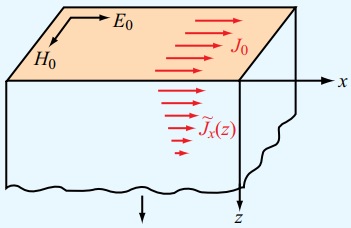
\includegraphics[width=\linewidth]{images/Plane Wave Propagation/ExponentiallyDecayingJ.png}
        \caption{Exponentially decaying $\phasor{J}_x(z)$.}
        \label{subfig:ExponentialDecayJ}
    \end{subfigure}
    \hfill
    \begin{subfigure}{0.48\linewidth}
        \centering
        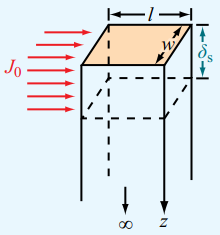
\includegraphics[width=0.6\linewidth]{images/Plane Wave Propagation/EquivalentJ0.png}
        \caption{Equivalent $J_0$ over skin depth $\delta_s$.}
        \label{subfig:EquivalentJ0}
    \end{subfigure}
    \caption{}
    \label{fig:ExponentialDecayJ}
\end{figure}

By the relation $\vec{J}=\sigma\vec{E}$, the current density is 
\begin{align}
    \vecphasor{J}(z) &= \uvec{x}\ \phasor{J}_x(z) = \uvec{x}\ \sigma E_0 e^{-\alpha z} e^{-j\beta z} = \uvec{x}\ J_0 e^{-\alpha z} e^{-j \beta z}
\end{align}
where $J_0 = \sigma E_0$. We can define the current density in terms of skin depths $\delta_s$ by using $\delta_s = 1/\alpha$ and the fact that $\alpha=\beta$ in a good conductor. 
\begin{align}
    \vecphasor{J}(z) &= \uvec{x}\ J_0 e^{-(1+j)z/\delta_s}
\end{align}
By this equation, we see clearly that the current density decays exponentially as the depth into the conductor increases. This phenomenon is called the \coltextit{skin effect}. The skin-depth influences the ac resistance. The surface impedance $Z_s$ is defined as the impedance $Z$ for a length and width $l = w = 1\ \text{m}$ and is given by 
\begin{empheq}[box=\eqnGreenBox]{equation}
    Z_s = \dfrac{1+j}{\sigma\delta_s} \qquad [\Omega]
\end{empheq}
The reactive part of $Z_s$ is positive, so $Z_s$ can be written as 
\begin{equation}
    Z_z = R_s j\omega L_s
\end{equation}
with 
\begin{align}
    R_s &= \dfrac{1}{\sigma\delta_s} = \sqrt{\dfrac{\pi f\mu}{\sigma}} \\ 
    L_s &= \dfrac{1}{\omega\sigma\delta_s} = \dfrac{1}{2} \sqrt{\dfrac{\mu}{\pi f\sigma}}
\end{align}
The ac resistance then for a slab of width $w$ and length $l$ is 
\begin{equation}
    R_\text{ac} = R_s \dfrac{l}{w} = \dfrac{1}{\sigma\delta_s w}
\end{equation}
For a coaxial cable, if $a$ and $b$ are the radii of the inner and outer conductors, respectively, the ac resistance per unit length is then 
\begin{empheq}[box=\eqnGreenBox]{equation}
    R_\text{ac, coax} = \dfrac{R_s}{2\pi} \left(\dfrac{1}{a} + \dfrac{1}{b} \right) \qquad [\Omega/\text{m}]
\end{empheq}

% ===========================================
% Power Density
% ===========================================
\section{Power Density}
The \coltextit{Poynting vector} represents the power per unit of area (power density) and is defined as 
\begin{equation}
    \vec{S} = \vec{E} \times \vec{H} \qquad [\text{W/m}^2] \label{eq:PoyntingVector}
\end{equation}
The power that flows through some surface area $A$ is then 
\begin{equation}
    P = \int\limits_A \vec{S} \cdot \uvec{n} \ dA \qquad [\text{W}]
\end{equation}
where $\uvec{n}$ is the normal unit vector to the surface. In Eq.\ (\ref{eq:PoyntingVector}), $\vec{E}$ and $\vec{H}$ are functions of time. We can express the time-averages power density $\vec{S}_\text{av}$ in terms of the fields in the phasor-domain: 
\begin{empheq}[box=\eqnGreenBox]{equation}
    \vec{S}_\text{av} = \dfrac{1}{2} \Re \{ \vecphasor{E} \times \vecphasor{H}^* \} \qquad [\text{W}/\text{m}^2]
\end{empheq}
In a \textit{lossless} medium, it can be shown that 
\begin{equation}
    \vec{S}_\text{av}(z) = \uvec{z}\ \dfrac{1}{2 \eta} (|E_{x_0}|^2 + |E_{y_0}|^2) = \uvec{z}\ \dfrac{|\vecphasor{E}|^2}{2\eta} \qquad [\text{W/m}^2]
\end{equation}
In a \textit{lossy} medium, 
\begin{equation}
    \vec{S}_\text{av}(z) = \uvec{z}\ \dfrac{|\vecphasor{E}|^2}{2|\eta_c|} e^{-2\alpha z} \cos\theta_\eta \qquad [\text{W/m}^2]
 \end{equation}
where $\eta_c = |\eta_c| e^{j\theta_\eta}$

% Microwave Networks --------------------------
\chapter{Wave Reflection and Transmission}
Some text... 

% Microwave Networks --------------------------
\input{chapters/MicrowaveNetworks}

\printbibliography

\end{document}
%%%%%%%%%%%%%%%%%%%%%%%%%%%%%%%%%%%%%%%%%%%%%%%%%%%%%%%
% END DOCUMENT
%%%%%%%%%%%%%%%%%%%%%%%%%%%%%%%%%%%%%%%%%%%%%%%%%%%%%%%
